% Options for packages loaded elsewhere
\PassOptionsToPackage{unicode}{hyperref}
\PassOptionsToPackage{hyphens}{url}
%
\documentclass[
]{article}
\title{mini\_project}
\author{Andrea Sama (A59010582)}
\date{10/27/2021}

\usepackage{amsmath,amssymb}
\usepackage{lmodern}
\usepackage{iftex}
\ifPDFTeX
  \usepackage[T1]{fontenc}
  \usepackage[utf8]{inputenc}
  \usepackage{textcomp} % provide euro and other symbols
\else % if luatex or xetex
  \usepackage{unicode-math}
  \defaultfontfeatures{Scale=MatchLowercase}
  \defaultfontfeatures[\rmfamily]{Ligatures=TeX,Scale=1}
\fi
% Use upquote if available, for straight quotes in verbatim environments
\IfFileExists{upquote.sty}{\usepackage{upquote}}{}
\IfFileExists{microtype.sty}{% use microtype if available
  \usepackage[]{microtype}
  \UseMicrotypeSet[protrusion]{basicmath} % disable protrusion for tt fonts
}{}
\makeatletter
\@ifundefined{KOMAClassName}{% if non-KOMA class
  \IfFileExists{parskip.sty}{%
    \usepackage{parskip}
  }{% else
    \setlength{\parindent}{0pt}
    \setlength{\parskip}{6pt plus 2pt minus 1pt}}
}{% if KOMA class
  \KOMAoptions{parskip=half}}
\makeatother
\usepackage{xcolor}
\IfFileExists{xurl.sty}{\usepackage{xurl}}{} % add URL line breaks if available
\IfFileExists{bookmark.sty}{\usepackage{bookmark}}{\usepackage{hyperref}}
\hypersetup{
  pdftitle={mini\_project},
  pdfauthor={Andrea Sama (A59010582)},
  hidelinks,
  pdfcreator={LaTeX via pandoc}}
\urlstyle{same} % disable monospaced font for URLs
\usepackage[margin=1in]{geometry}
\usepackage{color}
\usepackage{fancyvrb}
\newcommand{\VerbBar}{|}
\newcommand{\VERB}{\Verb[commandchars=\\\{\}]}
\DefineVerbatimEnvironment{Highlighting}{Verbatim}{commandchars=\\\{\}}
% Add ',fontsize=\small' for more characters per line
\usepackage{framed}
\definecolor{shadecolor}{RGB}{248,248,248}
\newenvironment{Shaded}{\begin{snugshade}}{\end{snugshade}}
\newcommand{\AlertTok}[1]{\textcolor[rgb]{0.94,0.16,0.16}{#1}}
\newcommand{\AnnotationTok}[1]{\textcolor[rgb]{0.56,0.35,0.01}{\textbf{\textit{#1}}}}
\newcommand{\AttributeTok}[1]{\textcolor[rgb]{0.77,0.63,0.00}{#1}}
\newcommand{\BaseNTok}[1]{\textcolor[rgb]{0.00,0.00,0.81}{#1}}
\newcommand{\BuiltInTok}[1]{#1}
\newcommand{\CharTok}[1]{\textcolor[rgb]{0.31,0.60,0.02}{#1}}
\newcommand{\CommentTok}[1]{\textcolor[rgb]{0.56,0.35,0.01}{\textit{#1}}}
\newcommand{\CommentVarTok}[1]{\textcolor[rgb]{0.56,0.35,0.01}{\textbf{\textit{#1}}}}
\newcommand{\ConstantTok}[1]{\textcolor[rgb]{0.00,0.00,0.00}{#1}}
\newcommand{\ControlFlowTok}[1]{\textcolor[rgb]{0.13,0.29,0.53}{\textbf{#1}}}
\newcommand{\DataTypeTok}[1]{\textcolor[rgb]{0.13,0.29,0.53}{#1}}
\newcommand{\DecValTok}[1]{\textcolor[rgb]{0.00,0.00,0.81}{#1}}
\newcommand{\DocumentationTok}[1]{\textcolor[rgb]{0.56,0.35,0.01}{\textbf{\textit{#1}}}}
\newcommand{\ErrorTok}[1]{\textcolor[rgb]{0.64,0.00,0.00}{\textbf{#1}}}
\newcommand{\ExtensionTok}[1]{#1}
\newcommand{\FloatTok}[1]{\textcolor[rgb]{0.00,0.00,0.81}{#1}}
\newcommand{\FunctionTok}[1]{\textcolor[rgb]{0.00,0.00,0.00}{#1}}
\newcommand{\ImportTok}[1]{#1}
\newcommand{\InformationTok}[1]{\textcolor[rgb]{0.56,0.35,0.01}{\textbf{\textit{#1}}}}
\newcommand{\KeywordTok}[1]{\textcolor[rgb]{0.13,0.29,0.53}{\textbf{#1}}}
\newcommand{\NormalTok}[1]{#1}
\newcommand{\OperatorTok}[1]{\textcolor[rgb]{0.81,0.36,0.00}{\textbf{#1}}}
\newcommand{\OtherTok}[1]{\textcolor[rgb]{0.56,0.35,0.01}{#1}}
\newcommand{\PreprocessorTok}[1]{\textcolor[rgb]{0.56,0.35,0.01}{\textit{#1}}}
\newcommand{\RegionMarkerTok}[1]{#1}
\newcommand{\SpecialCharTok}[1]{\textcolor[rgb]{0.00,0.00,0.00}{#1}}
\newcommand{\SpecialStringTok}[1]{\textcolor[rgb]{0.31,0.60,0.02}{#1}}
\newcommand{\StringTok}[1]{\textcolor[rgb]{0.31,0.60,0.02}{#1}}
\newcommand{\VariableTok}[1]{\textcolor[rgb]{0.00,0.00,0.00}{#1}}
\newcommand{\VerbatimStringTok}[1]{\textcolor[rgb]{0.31,0.60,0.02}{#1}}
\newcommand{\WarningTok}[1]{\textcolor[rgb]{0.56,0.35,0.01}{\textbf{\textit{#1}}}}
\usepackage{longtable,booktabs,array}
\usepackage{calc} % for calculating minipage widths
% Correct order of tables after \paragraph or \subparagraph
\usepackage{etoolbox}
\makeatletter
\patchcmd\longtable{\par}{\if@noskipsec\mbox{}\fi\par}{}{}
\makeatother
% Allow footnotes in longtable head/foot
\IfFileExists{footnotehyper.sty}{\usepackage{footnotehyper}}{\usepackage{footnote}}
\makesavenoteenv{longtable}
\usepackage{graphicx}
\makeatletter
\def\maxwidth{\ifdim\Gin@nat@width>\linewidth\linewidth\else\Gin@nat@width\fi}
\def\maxheight{\ifdim\Gin@nat@height>\textheight\textheight\else\Gin@nat@height\fi}
\makeatother
% Scale images if necessary, so that they will not overflow the page
% margins by default, and it is still possible to overwrite the defaults
% using explicit options in \includegraphics[width, height, ...]{}
\setkeys{Gin}{width=\maxwidth,height=\maxheight,keepaspectratio}
% Set default figure placement to htbp
\makeatletter
\def\fps@figure{htbp}
\makeatother
\setlength{\emergencystretch}{3em} % prevent overfull lines
\providecommand{\tightlist}{%
  \setlength{\itemsep}{0pt}\setlength{\parskip}{0pt}}
\setcounter{secnumdepth}{-\maxdimen} % remove section numbering
\ifLuaTeX
  \usepackage{selnolig}  % disable illegal ligatures
\fi

\begin{document}
\maketitle

\begin{Shaded}
\begin{Highlighting}[]
\CommentTok{\#read.csv("WisconsinCancer.csv")}
\end{Highlighting}
\end{Shaded}

\hypertarget{save-your-input-data-file-into-your-project-directory}{%
\section{Save your input data file into your Project
directory}\label{save-your-input-data-file-into-your-project-directory}}

\begin{Shaded}
\begin{Highlighting}[]
\NormalTok{fna.data }\OtherTok{\textless{}{-}} \StringTok{"WisconsinCancer.csv"}
\end{Highlighting}
\end{Shaded}

\hypertarget{complete-the-following-code-to-input-the-data-and-store-as-wisc.df}{%
\section{Complete the following code to input the data and store as
wisc.df}\label{complete-the-following-code-to-input-the-data-and-store-as-wisc.df}}

\begin{Shaded}
\begin{Highlighting}[]
\NormalTok{wisc.df }\OtherTok{\textless{}{-}} \FunctionTok{read.csv}\NormalTok{(fna.data, }\AttributeTok{row.names=}\DecValTok{1}\NormalTok{)}
\end{Highlighting}
\end{Shaded}

\begin{Shaded}
\begin{Highlighting}[]
\CommentTok{\# We can use {-}1 here to remove the first column}
\NormalTok{wisc.data }\OtherTok{\textless{}{-}}\NormalTok{ wisc.df[,}\SpecialCharTok{{-}}\DecValTok{1}\NormalTok{]}
\end{Highlighting}
\end{Shaded}

\begin{Shaded}
\begin{Highlighting}[]
\CommentTok{\#Setting diagnosis as a factor}
\NormalTok{diagnosis }\OtherTok{\textless{}{-}} \FunctionTok{as.factor}\NormalTok{(wisc.df}\SpecialCharTok{$}\NormalTok{diagnosis)}
\NormalTok{diagnosis}
\end{Highlighting}
\end{Shaded}

\begin{verbatim}
##   [1] M M M M M M M M M M M M M M M M M M M B B B M M M M M M M M M M M M M M M
##  [38] B M M M M M M M M B M B B B B B M M B M M B B B B M B M M B B B B M B M M
##  [75] B M B M M B B B M M B M M M B B B M B B M M B B B M M B B B B M B B M B B
## [112] B B B B B B M M M B M M B B B M M B M B M M B M M B B M B B M B B B B M B
## [149] B B B B B B B B M B B B B M M B M B B M M B B M M B B B B M B B M M M B M
## [186] B M B B B M B B M M B M M M M B M M M B M B M B B M B M M M M B B M M B B
## [223] B M B B B B B M M B B M B B M M B M B B B B M B B B B B M B M M M M M M M
## [260] M M M M M M M B B B B B B M B M B B M B B M B M M B B B B B B B B B B B B
## [297] B M B B M B M B B B B B B B B B B B B B B M B B B M B M B B B B M M M B B
## [334] B B M B M B M B B B M B B B B B B B M M M B B B B B B B B B B B M M B M M
## [371] M B M M B B B B B M B B B B B M B B B M B B M M B B B B B B M B B B B B B
## [408] B M B B B B B M B B M B B B B B B B B B B B B M B M M B M B B B B B M B B
## [445] M B M B B M B M B B B B B B B B M M B B B B B B M B B B B B B B B B B M B
## [482] B B B B B B M B M B B M B B B B B M M B M B M B B B B B M B B M B M B M M
## [519] B B B M B B B B B B B B B B B M B M M B B B B B B B B B B B B B B B B B B
## [556] B B B B B B B M M M M M M B
## Levels: B M
\end{verbatim}

\#Question 1: How many observations are there in this dataset?

\begin{Shaded}
\begin{Highlighting}[]
\FunctionTok{nrow}\NormalTok{(wisc.data)}
\end{Highlighting}
\end{Shaded}

\begin{verbatim}
## [1] 569
\end{verbatim}

\#Question 2: How many observations have a malignant diagnosis?

\begin{Shaded}
\begin{Highlighting}[]
\FunctionTok{table}\NormalTok{(diagnosis)}
\end{Highlighting}
\end{Shaded}

\begin{verbatim}
## diagnosis
##   B   M 
## 357 212
\end{verbatim}

\#Question 3: How many variables/features in the data are suffixed with
\_mean?

\begin{Shaded}
\begin{Highlighting}[]
\FunctionTok{grepl}\NormalTok{(}\StringTok{"\_mean"}\NormalTok{, }\FunctionTok{colnames}\NormalTok{(wisc.data))}
\end{Highlighting}
\end{Shaded}

\begin{verbatim}
##  [1]  TRUE  TRUE  TRUE  TRUE  TRUE  TRUE  TRUE  TRUE  TRUE  TRUE FALSE FALSE
## [13] FALSE FALSE FALSE FALSE FALSE FALSE FALSE FALSE FALSE FALSE FALSE FALSE
## [25] FALSE FALSE FALSE FALSE FALSE FALSE
\end{verbatim}

There are 10 that are suffixed with mean

\begin{Shaded}
\begin{Highlighting}[]
\CommentTok{\# Check column means and standard deviations}
\FunctionTok{colMeans}\NormalTok{(wisc.data)}
\end{Highlighting}
\end{Shaded}

\begin{verbatim}
##             radius_mean            texture_mean          perimeter_mean 
##            1.412729e+01            1.928965e+01            9.196903e+01 
##               area_mean         smoothness_mean        compactness_mean 
##            6.548891e+02            9.636028e-02            1.043410e-01 
##          concavity_mean     concave.points_mean           symmetry_mean 
##            8.879932e-02            4.891915e-02            1.811619e-01 
##  fractal_dimension_mean               radius_se              texture_se 
##            6.279761e-02            4.051721e-01            1.216853e+00 
##            perimeter_se                 area_se           smoothness_se 
##            2.866059e+00            4.033708e+01            7.040979e-03 
##          compactness_se            concavity_se       concave.points_se 
##            2.547814e-02            3.189372e-02            1.179614e-02 
##             symmetry_se    fractal_dimension_se            radius_worst 
##            2.054230e-02            3.794904e-03            1.626919e+01 
##           texture_worst         perimeter_worst              area_worst 
##            2.567722e+01            1.072612e+02            8.805831e+02 
##        smoothness_worst       compactness_worst         concavity_worst 
##            1.323686e-01            2.542650e-01            2.721885e-01 
##    concave.points_worst          symmetry_worst fractal_dimension_worst 
##            1.146062e-01            2.900756e-01            8.394582e-02
\end{verbatim}

\begin{Shaded}
\begin{Highlighting}[]
\FunctionTok{apply}\NormalTok{(wisc.data,}\DecValTok{2}\NormalTok{,sd)}
\end{Highlighting}
\end{Shaded}

\begin{verbatim}
##             radius_mean            texture_mean          perimeter_mean 
##            3.524049e+00            4.301036e+00            2.429898e+01 
##               area_mean         smoothness_mean        compactness_mean 
##            3.519141e+02            1.406413e-02            5.281276e-02 
##          concavity_mean     concave.points_mean           symmetry_mean 
##            7.971981e-02            3.880284e-02            2.741428e-02 
##  fractal_dimension_mean               radius_se              texture_se 
##            7.060363e-03            2.773127e-01            5.516484e-01 
##            perimeter_se                 area_se           smoothness_se 
##            2.021855e+00            4.549101e+01            3.002518e-03 
##          compactness_se            concavity_se       concave.points_se 
##            1.790818e-02            3.018606e-02            6.170285e-03 
##             symmetry_se    fractal_dimension_se            radius_worst 
##            8.266372e-03            2.646071e-03            4.833242e+00 
##           texture_worst         perimeter_worst              area_worst 
##            6.146258e+00            3.360254e+01            5.693570e+02 
##        smoothness_worst       compactness_worst         concavity_worst 
##            2.283243e-02            1.573365e-01            2.086243e-01 
##    concave.points_worst          symmetry_worst fractal_dimension_worst 
##            6.573234e-02            6.186747e-02            1.806127e-02
\end{verbatim}

\begin{Shaded}
\begin{Highlighting}[]
\CommentTok{\# Perform PCA on wisc.data by completing the following code}
\NormalTok{wisc.pr }\OtherTok{\textless{}{-}} \FunctionTok{prcomp}\NormalTok{(}\FunctionTok{scale}\NormalTok{(wisc.data))}
\end{Highlighting}
\end{Shaded}

\begin{Shaded}
\begin{Highlighting}[]
\FunctionTok{summary}\NormalTok{(wisc.pr)}
\end{Highlighting}
\end{Shaded}

\begin{verbatim}
## Importance of components:
##                           PC1    PC2     PC3     PC4     PC5     PC6     PC7
## Standard deviation     3.6444 2.3857 1.67867 1.40735 1.28403 1.09880 0.82172
## Proportion of Variance 0.4427 0.1897 0.09393 0.06602 0.05496 0.04025 0.02251
## Cumulative Proportion  0.4427 0.6324 0.72636 0.79239 0.84734 0.88759 0.91010
##                            PC8    PC9    PC10   PC11    PC12    PC13    PC14
## Standard deviation     0.69037 0.6457 0.59219 0.5421 0.51104 0.49128 0.39624
## Proportion of Variance 0.01589 0.0139 0.01169 0.0098 0.00871 0.00805 0.00523
## Cumulative Proportion  0.92598 0.9399 0.95157 0.9614 0.97007 0.97812 0.98335
##                           PC15    PC16    PC17    PC18    PC19    PC20   PC21
## Standard deviation     0.30681 0.28260 0.24372 0.22939 0.22244 0.17652 0.1731
## Proportion of Variance 0.00314 0.00266 0.00198 0.00175 0.00165 0.00104 0.0010
## Cumulative Proportion  0.98649 0.98915 0.99113 0.99288 0.99453 0.99557 0.9966
##                           PC22    PC23   PC24    PC25    PC26    PC27    PC28
## Standard deviation     0.16565 0.15602 0.1344 0.12442 0.09043 0.08307 0.03987
## Proportion of Variance 0.00091 0.00081 0.0006 0.00052 0.00027 0.00023 0.00005
## Cumulative Proportion  0.99749 0.99830 0.9989 0.99942 0.99969 0.99992 0.99997
##                           PC29    PC30
## Standard deviation     0.02736 0.01153
## Proportion of Variance 0.00002 0.00000
## Cumulative Proportion  1.00000 1.00000
\end{verbatim}

\#Question 4: From your results, what proportion of the original
variance is captured by the first principal components (PC1)?

44.27\%

\#Question 5: How many principal components (PCs) are required to
describe at least 70\% of the original variance in the data?

Three of the PCs are required to describe at least 70\% of the original
variance, as the PC3 cumulative proportion is reported as 72\%.

\#Q6. How many principal components (PCs) are required to describe at
least 90\% of the original variance in the data?

Seven PCs are required to describe at least 90\% of the original
variance, PC7's cumulative proportion is 91\%.

\#Plot this:

\begin{Shaded}
\begin{Highlighting}[]
\FunctionTok{biplot}\NormalTok{(wisc.pr)}
\end{Highlighting}
\end{Shaded}

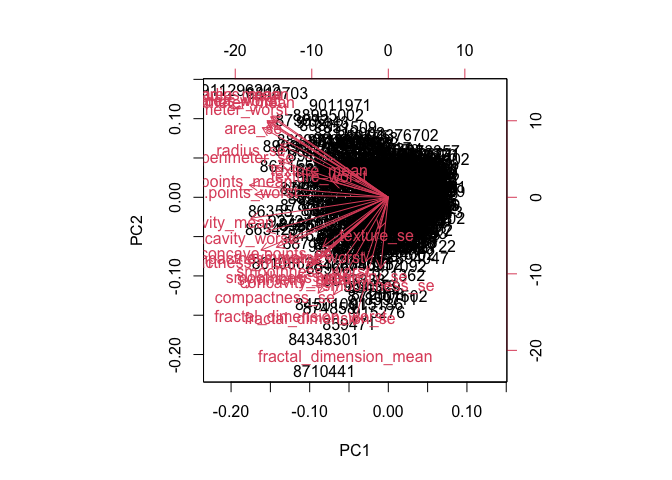
\includegraphics{test_files/figure-latex/unnamed-chunk-12-1.pdf} \#Q7.
What stands out to you about this plot? Is it easy or difficult to
understand? Why?

This plot is not easy to understand, it is very crowded and I don't know
what anything means.

\#Making a better plot:

\begin{Shaded}
\begin{Highlighting}[]
\CommentTok{\# Scatter plot observations by components 1 and 2}
\FunctionTok{plot}\NormalTok{(wisc.pr}\SpecialCharTok{$}\NormalTok{x[,}\DecValTok{1}\SpecialCharTok{:}\DecValTok{2}\NormalTok{], }\AttributeTok{col =}\NormalTok{ diagnosis , }
     \AttributeTok{xlab =} \StringTok{"PC1"}\NormalTok{, }\AttributeTok{ylab =} \StringTok{"PC2"}\NormalTok{)}
\end{Highlighting}
\end{Shaded}

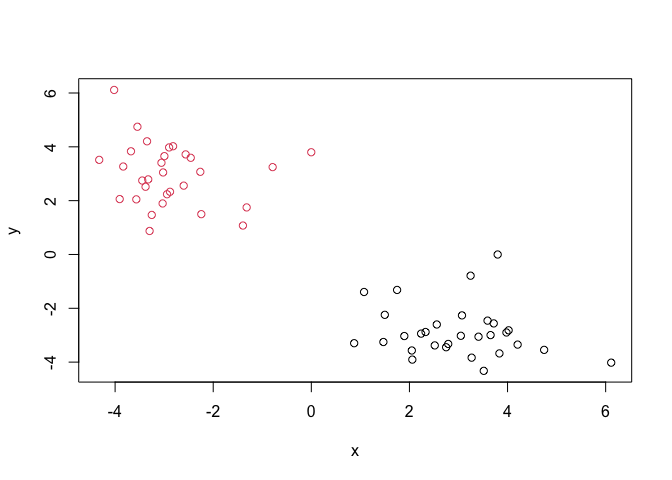
\includegraphics{test_files/figure-latex/unnamed-chunk-13-1.pdf}

\#Question 8: Generate a similar plot for principal components 1 and 3.
What do you notice about these plots?

\begin{Shaded}
\begin{Highlighting}[]
\NormalTok{wisc.pr}
\end{Highlighting}
\end{Shaded}

\begin{verbatim}
## Standard deviations (1, .., p=30):
##  [1] 3.64439401 2.38565601 1.67867477 1.40735229 1.28402903 1.09879780
##  [7] 0.82171778 0.69037464 0.64567392 0.59219377 0.54213992 0.51103950
## [13] 0.49128148 0.39624453 0.30681422 0.28260007 0.24371918 0.22938785
## [19] 0.22243559 0.17652026 0.17312681 0.16564843 0.15601550 0.13436892
## [25] 0.12442376 0.09043030 0.08306903 0.03986650 0.02736427 0.01153451
## 
## Rotation (n x k) = (30 x 30):
##                                 PC1          PC2          PC3          PC4
## radius_mean             -0.21890244  0.233857132 -0.008531243  0.041408962
## texture_mean            -0.10372458  0.059706088  0.064549903 -0.603050001
## perimeter_mean          -0.22753729  0.215181361 -0.009314220  0.041983099
## area_mean               -0.22099499  0.231076711  0.028699526  0.053433795
## smoothness_mean         -0.14258969 -0.186113023 -0.104291904  0.159382765
## compactness_mean        -0.23928535 -0.151891610 -0.074091571  0.031794581
## concavity_mean          -0.25840048 -0.060165363  0.002733838  0.019122753
## concave.points_mean     -0.26085376  0.034767500 -0.025563541  0.065335944
## symmetry_mean           -0.13816696 -0.190348770 -0.040239936  0.067124984
## fractal_dimension_mean  -0.06436335 -0.366575471 -0.022574090  0.048586765
## radius_se               -0.20597878  0.105552152  0.268481387  0.097941242
## texture_se              -0.01742803 -0.089979682  0.374633665 -0.359855528
## perimeter_se            -0.21132592  0.089457234  0.266645367  0.088992415
## area_se                 -0.20286964  0.152292628  0.216006528  0.108205039
## smoothness_se           -0.01453145 -0.204430453  0.308838979  0.044664180
## compactness_se          -0.17039345 -0.232715896  0.154779718 -0.027469363
## concavity_se            -0.15358979 -0.197207283  0.176463743  0.001316880
## concave.points_se       -0.18341740 -0.130321560  0.224657567  0.074067335
## symmetry_se             -0.04249842 -0.183848000  0.288584292  0.044073351
## fractal_dimension_se    -0.10256832 -0.280092027  0.211503764  0.015304750
## radius_worst            -0.22799663  0.219866379 -0.047506990  0.015417240
## texture_worst           -0.10446933  0.045467298 -0.042297823 -0.632807885
## perimeter_worst         -0.23663968  0.199878428 -0.048546508  0.013802794
## area_worst              -0.22487053  0.219351858 -0.011902318  0.025894749
## smoothness_worst        -0.12795256 -0.172304352 -0.259797613  0.017652216
## compactness_worst       -0.21009588 -0.143593173 -0.236075625 -0.091328415
## concavity_worst         -0.22876753 -0.097964114 -0.173057335 -0.073951180
## concave.points_worst    -0.25088597  0.008257235 -0.170344076  0.006006996
## symmetry_worst          -0.12290456 -0.141883349 -0.271312642 -0.036250695
## fractal_dimension_worst -0.13178394 -0.275339469 -0.232791313 -0.077053470
##                                  PC5           PC6           PC7          PC8
## radius_mean             -0.037786354  0.0187407904 -0.1240883403  0.007452296
## texture_mean             0.049468850 -0.0321788366  0.0113995382 -0.130674825
## perimeter_mean          -0.037374663  0.0173084449 -0.1144770573  0.018687258
## area_mean               -0.010331251 -0.0018877480 -0.0516534275 -0.034673604
## smoothness_mean          0.365088528 -0.2863744966 -0.1406689928  0.288974575
## compactness_mean        -0.011703971 -0.0141309489  0.0309184960  0.151396350
## concavity_mean          -0.086375412 -0.0093441809 -0.1075204434  0.072827285
## concave.points_mean      0.043861025 -0.0520499505 -0.1504822142  0.152322414
## symmetry_mean            0.305941428  0.3564584607 -0.0938911345  0.231530989
## fractal_dimension_mean   0.044424360 -0.1194306679  0.2957600240  0.177121441
## radius_se                0.154456496 -0.0256032561  0.3124900373 -0.022539967
## texture_se               0.191650506 -0.0287473145 -0.0907553556  0.475413139
## perimeter_se             0.120990220  0.0018107150  0.3146403902  0.011896690
## area_se                  0.127574432 -0.0428639079  0.3466790028 -0.085805135
## smoothness_se            0.232065676 -0.3429173935 -0.2440240556 -0.573410232
## compactness_se          -0.279968156  0.0691975186  0.0234635340 -0.117460157
## concavity_se            -0.353982091  0.0563432386 -0.2088237897 -0.060566501
## concave.points_se       -0.195548089 -0.0312244482 -0.3696459369  0.108319309
## symmetry_se              0.252868765  0.4902456426 -0.0803822539 -0.220149279
## fractal_dimension_se    -0.263297438 -0.0531952674  0.1913949726 -0.011168188
## radius_worst             0.004406592 -0.0002906849 -0.0097099360 -0.042619416
## texture_worst            0.092883400 -0.0500080613  0.0098707439 -0.036251636
## perimeter_worst         -0.007454151  0.0085009872 -0.0004457267 -0.030558534
## area_worst               0.027390903 -0.0251643821  0.0678316595 -0.079394246
## smoothness_worst         0.324435445 -0.3692553703 -0.1088308865 -0.205852191
## compactness_worst       -0.121804107  0.0477057929  0.1404729381 -0.084019659
## concavity_worst         -0.188518727  0.0283792555 -0.0604880561 -0.072467871
## concave.points_worst    -0.043332069 -0.0308734498 -0.1679666187  0.036170795
## symmetry_worst           0.244558663  0.4989267845 -0.0184906298 -0.228225053
## fractal_dimension_worst -0.094423351 -0.0802235245  0.3746576261 -0.048360667
##                                  PC9         PC10        PC11         PC12
## radius_mean             -0.223109764  0.095486443 -0.04147149  0.051067457
## texture_mean             0.112699390  0.240934066  0.30224340  0.254896423
## perimeter_mean          -0.223739213  0.086385615 -0.01678264  0.038926106
## area_mean               -0.195586014  0.074956489 -0.11016964  0.065437508
## smoothness_mean          0.006424722 -0.069292681  0.13702184  0.316727211
## compactness_mean        -0.167841425  0.012936200  0.30800963 -0.104017044
## concavity_mean           0.040591006 -0.135602298 -0.12419024  0.065653480
## concave.points_mean     -0.111971106  0.008054528  0.07244603  0.042589267
## symmetry_mean            0.256040084  0.572069479 -0.16305408 -0.288865504
## fractal_dimension_mean  -0.123740789  0.081103207  0.03804827  0.236358988
## radius_se                0.249985002 -0.049547594  0.02535702 -0.016687915
## texture_se              -0.246645397 -0.289142742 -0.34494446 -0.306160423
## perimeter_se             0.227154024 -0.114508236  0.16731877 -0.101446828
## area_se                  0.229160015 -0.091927889 -0.05161946 -0.017679218
## smoothness_se           -0.141924890  0.160884609 -0.08420621 -0.294710053
## compactness_se          -0.145322810  0.043504866  0.20688568 -0.263456509
## concavity_se             0.358107079 -0.141276243 -0.34951794  0.251146975
## concave.points_se        0.272519886  0.086240847  0.34237591 -0.006458751
## symmetry_se             -0.304077200 -0.316529830  0.18784404  0.320571348
## fractal_dimension_se    -0.213722716  0.367541918 -0.25062479  0.276165974
## radius_worst            -0.112141463  0.077361643 -0.10506733  0.039679665
## texture_worst            0.103341204  0.029550941 -0.01315727  0.079797450
## perimeter_worst         -0.109614364  0.050508334 -0.05107628 -0.008987738
## area_worst              -0.080732461  0.069921152 -0.18459894  0.048088657
## smoothness_worst         0.112315904 -0.128304659 -0.14389035  0.056514866
## compactness_worst       -0.100677822 -0.172133632  0.19742047 -0.371662503
## concavity_worst          0.161908621 -0.311638520 -0.18501676 -0.087034532
## concave.points_worst     0.060488462 -0.076648291  0.11777205 -0.068125354
## symmetry_worst           0.064637806 -0.029563075 -0.15756025  0.044033503
## fractal_dimension_worst -0.134174175  0.012609579 -0.11828355 -0.034731693
##                                PC13         PC14         PC15        PC16
## radius_mean              0.01196721  0.059506135 -0.051118775 -0.15058388
## texture_mean             0.20346133 -0.021560100 -0.107922421 -0.15784196
## perimeter_mean           0.04410950  0.048513812 -0.039902936 -0.11445396
## area_mean                0.06737574  0.010830829  0.013966907 -0.13244803
## smoothness_mean          0.04557360  0.445064860 -0.118143364 -0.20461325
## compactness_mean         0.22928130  0.008101057  0.230899962  0.17017837
## concavity_mean           0.38709081 -0.189358699 -0.128283732  0.26947021
## concave.points_mean      0.13213810 -0.244794768 -0.217099194  0.38046410
## symmetry_mean            0.18993367  0.030738856 -0.073961707 -0.16466159
## fractal_dimension_mean   0.10623908 -0.377078865  0.517975705 -0.04079279
## radius_se               -0.06819523  0.010347413 -0.110050711  0.05890572
## texture_se              -0.16822238 -0.010849347  0.032752721 -0.03450040
## perimeter_se            -0.03784399 -0.045523718 -0.008268089  0.02651665
## area_se                  0.05606493  0.083570718 -0.046024366  0.04115323
## smoothness_se            0.15044143 -0.201152530  0.018559465 -0.05803906
## compactness_se           0.01004017  0.491755932  0.168209315  0.18983090
## concavity_se             0.15878319  0.134586924  0.250471408 -0.12542065
## concave.points_se       -0.49402674 -0.199666719  0.062079344 -0.19881035
## symmetry_se              0.01033274 -0.046864383 -0.113383199 -0.15771150
## fractal_dimension_se    -0.24045832  0.145652466 -0.353232211  0.26855388
## radius_worst            -0.13789053  0.023101281  0.166567074 -0.08156057
## texture_worst           -0.08014543  0.053430792  0.101115399  0.18555785
## perimeter_worst         -0.09696571  0.012219382  0.182755198 -0.05485705
## area_worst              -0.10116061 -0.006685465  0.314993600 -0.09065339
## smoothness_worst        -0.20513034  0.162235443  0.046125866  0.14555166
## compactness_worst        0.01227931  0.166470250 -0.049956014 -0.15373486
## concavity_worst          0.21798433 -0.066798931 -0.204835886 -0.21502195
## concave.points_worst    -0.25438749 -0.276418891 -0.169499607  0.17814174
## symmetry_worst          -0.25653491  0.005355574  0.139888394  0.25789401
## fractal_dimension_worst -0.17281424 -0.212104110 -0.256173195 -0.40555649
##                                 PC17          PC18        PC19         PC20
## radius_mean              0.202924255  0.1467123385  0.22538466 -0.049698664
## texture_mean            -0.038706119 -0.0411029851  0.02978864 -0.244134993
## perimeter_mean           0.194821310  0.1583174548  0.23959528 -0.017665012
## area_mean                0.255705763  0.2661681046 -0.02732219 -0.090143762
## smoothness_mean          0.167929914 -0.3522268017 -0.16456584  0.017100960
## compactness_mean        -0.020307708  0.0077941384  0.28422236  0.488686329
## concavity_mean          -0.001598353 -0.0269681105  0.00226636 -0.033387086
## concave.points_mean      0.034509509 -0.0828277367 -0.15497236 -0.235407606
## symmetry_mean           -0.191737848  0.1733977905 -0.05881116  0.026069156
## fractal_dimension_mean   0.050225246  0.0878673570 -0.05815705 -0.175637222
## radius_se               -0.139396866 -0.2362165319  0.17588331 -0.090800503
## texture_se               0.043963016 -0.0098586620  0.03600985 -0.071659988
## perimeter_se            -0.024635639 -0.0259288003  0.36570154 -0.177250625
## area_se                  0.334418173  0.3049069032 -0.41657231  0.274201148
## smoothness_se            0.139595006 -0.2312599432 -0.01326009  0.090061477
## compactness_se          -0.008246477  0.1004742346 -0.24244818 -0.461098220
## concavity_se             0.084616716 -0.0001954852  0.12638102  0.066946174
## concave.points_se        0.108132263  0.0460549116 -0.01216430  0.068868294
## symmetry_se             -0.274059129  0.1870147640 -0.08903929  0.107385289
## fractal_dimension_se    -0.122733398 -0.0598230982  0.08660084  0.222345297
## radius_worst            -0.240049982 -0.2161013526  0.01366130 -0.005626909
## texture_worst            0.069365185  0.0583984505 -0.07586693  0.300599798
## perimeter_worst         -0.234164147 -0.1885435919  0.09081325  0.011003858
## area_worst              -0.273399584 -0.1420648558 -0.41004720  0.060047387
## smoothness_worst        -0.278030197  0.5015516751  0.23451384 -0.129723903
## compactness_worst       -0.004037123 -0.0735745143  0.02020070  0.229280589
## concavity_worst         -0.191313419 -0.1039079796 -0.04578612 -0.046482792
## concave.points_worst    -0.075485316  0.0758138963 -0.26022962  0.033022340
## symmetry_worst           0.430658116 -0.2787138431  0.11725053 -0.116759236
## fractal_dimension_worst  0.159394300  0.0235647497 -0.01149448 -0.104991974
##                                  PC21        PC22          PC23        PC24
## radius_mean             -0.0685700057 -0.07292890 -0.0985526942 -0.18257944
## texture_mean             0.4483694667 -0.09480063 -0.0005549975  0.09878679
## perimeter_mean          -0.0697690429 -0.07516048 -0.0402447050 -0.11664888
## area_mean               -0.0184432785 -0.09756578  0.0077772734  0.06984834
## smoothness_mean         -0.1194917473 -0.06382295 -0.0206657211  0.06869742
## compactness_mean         0.1926213963  0.09807756  0.0523603957 -0.10413552
## concavity_mean           0.0055717533  0.18521200  0.3248703785  0.04474106
## concave.points_mean     -0.0094238187  0.31185243 -0.0514087968  0.08402770
## symmetry_mean           -0.0869384844  0.01840673 -0.0512005770  0.01933947
## fractal_dimension_mean  -0.0762718362 -0.28786888 -0.0846898562 -0.13326055
## radius_se                0.0863867747  0.15027468 -0.2641253170 -0.55870157
## texture_se               0.2170719674 -0.04845693 -0.0008738805  0.02426730
## perimeter_se            -0.3049501584 -0.15935280  0.0900742110  0.51675039
## area_se                  0.1925877857 -0.06423262  0.0982150746 -0.02246072
## smoothness_se           -0.0720987261 -0.05054490 -0.0598177179  0.01563119
## compactness_se          -0.1403865724  0.04528769  0.0091038710 -0.12177779
## concavity_se             0.0630479298  0.20521269 -0.3875423290  0.18820504
## concave.points_se        0.0343753236  0.07254538  0.3517550738 -0.10966898
## symmetry_se             -0.0976995265  0.08465443 -0.0423628949  0.00322620
## fractal_dimension_se     0.0628432814 -0.24470508  0.0857810992  0.07519442
## radius_worst             0.0072938995  0.09629821 -0.0556767923 -0.15683037
## texture_worst           -0.5944401434  0.11111202 -0.0089228997 -0.11848460
## perimeter_worst         -0.0920235990 -0.01722163  0.0633448296  0.23711317
## area_worst               0.1467901315  0.09695982  0.1908896250  0.14406303
## smoothness_worst         0.1648492374  0.06825409  0.0936901494 -0.01099014
## compactness_worst        0.1813748671 -0.02967641 -0.1479209247  0.18674995
## concavity_worst         -0.1321005945 -0.46042619  0.2864331353 -0.28885257
## concave.points_worst     0.0008860815 -0.29984056 -0.5675277966  0.10734024
## symmetry_worst           0.1627085487 -0.09714484  0.1213434508 -0.01438181
## fractal_dimension_worst -0.0923439434  0.46947115  0.0076253382  0.03782545
##                                PC25         PC26         PC27          PC28
## radius_mean             -0.01922650 -0.129476396 -0.131526670  2.111940e-01
## texture_mean             0.08474593 -0.024556664 -0.017357309 -6.581146e-05
## perimeter_mean           0.02701541 -0.125255946 -0.115415423  8.433827e-02
## area_mean               -0.21004078  0.362727403  0.466612477 -2.725083e-01
## smoothness_mean          0.02895489 -0.037003686  0.069689923  1.479269e-03
## compactness_mean         0.39662323  0.262808474  0.097748705 -5.462767e-03
## concavity_mean          -0.09697732 -0.548876170  0.364808397  4.553864e-02
## concave.points_mean     -0.18645160  0.387643377 -0.454699351 -8.883097e-03
## symmetry_mean           -0.02458369 -0.016044038 -0.015164835  1.433026e-03
## fractal_dimension_mean  -0.20722186 -0.097404839 -0.101244946 -6.311687e-03
## radius_se               -0.17493043  0.049977080  0.212982901 -1.922239e-01
## texture_se               0.05698648 -0.011237242 -0.010092889 -5.622611e-03
## perimeter_se             0.07292764  0.103653282  0.041691553  2.631919e-01
## area_se                  0.13185041 -0.155304589 -0.313358657 -4.206811e-02
## smoothness_se            0.03121070 -0.007717557 -0.009052154  9.792963e-03
## compactness_se           0.17316455 -0.049727632  0.046536088 -1.539555e-02
## concavity_se             0.01593998  0.091454968 -0.084224797  5.820978e-03
## concave.points_se       -0.12954655 -0.017941919 -0.011165509 -2.900930e-02
## symmetry_se             -0.01951493 -0.017267849 -0.019975983 -7.636526e-03
## fractal_dimension_se    -0.08417120  0.035488974 -0.012036564  1.975646e-02
## radius_worst             0.07070972 -0.197054744 -0.178666740  4.126396e-01
## texture_worst           -0.11818972  0.036469433  0.021410694 -3.902509e-04
## perimeter_worst          0.11803403 -0.244103670 -0.241031046 -7.286809e-01
## area_worst              -0.03828995  0.231359525  0.237162466  2.389603e-01
## smoothness_worst        -0.04796476  0.012602464 -0.040853568 -1.535248e-03
## compactness_worst       -0.62438494 -0.100463424 -0.070505414  4.869182e-02
## concavity_worst          0.11577034  0.266853781 -0.142905801 -1.764090e-02
## concave.points_worst     0.26319634 -0.133574507  0.230901389  2.247567e-02
## symmetry_worst           0.04529962  0.028184296  0.022790444  4.920481e-03
## fractal_dimension_worst  0.28013348  0.004520482  0.059985998 -2.356214e-02
##                                  PC29          PC30
## radius_mean              2.114605e-01  0.7024140910
## texture_mean            -1.053393e-02  0.0002736610
## perimeter_mean           3.838261e-01 -0.6898969685
## area_mean               -4.227949e-01 -0.0329473482
## smoothness_mean         -3.434667e-03 -0.0048474577
## compactness_mean        -4.101677e-02  0.0446741863
## concavity_mean          -1.001479e-02  0.0251386661
## concave.points_mean     -4.206949e-03 -0.0010772653
## symmetry_mean           -7.569862e-03 -0.0012803794
## fractal_dimension_mean   7.301433e-03 -0.0047556848
## radius_se                1.184421e-01 -0.0087110937
## texture_se              -8.776279e-03 -0.0010710392
## perimeter_se            -6.100219e-03  0.0137293906
## area_se                 -8.592591e-02  0.0011053260
## smoothness_se            1.776386e-03 -0.0016082109
## compactness_se           3.158134e-03  0.0019156224
## concavity_se             1.607852e-02 -0.0089265265
## concave.points_se       -2.393779e-02 -0.0021601973
## symmetry_se             -5.223292e-03  0.0003293898
## fractal_dimension_se    -8.341912e-03  0.0017989568
## radius_worst            -6.357249e-01 -0.1356430561
## texture_worst            1.723549e-02  0.0010205360
## perimeter_worst          2.292180e-02  0.0797438536
## area_worst               4.449359e-01  0.0397422838
## smoothness_worst         7.385492e-03  0.0045832773
## compactness_worst        3.566904e-06 -0.0128415624
## concavity_worst         -1.267572e-02  0.0004021392
## concave.points_worst     3.524045e-02 -0.0022884418
## symmetry_worst           1.340423e-02  0.0003954435
## fractal_dimension_worst  1.147766e-02  0.0018942925
\end{verbatim}

\begin{Shaded}
\begin{Highlighting}[]
\FunctionTok{plot}\NormalTok{(wisc.pr}\SpecialCharTok{$}\NormalTok{x[,}\FunctionTok{c}\NormalTok{(}\DecValTok{1}\NormalTok{,}\DecValTok{3}\NormalTok{) ], }\AttributeTok{col =}\NormalTok{ diagnosis, }
     \AttributeTok{xlab =} \StringTok{"PC1"}\NormalTok{, }\AttributeTok{ylab =} \StringTok{"PC3"}\NormalTok{)}
\end{Highlighting}
\end{Shaded}

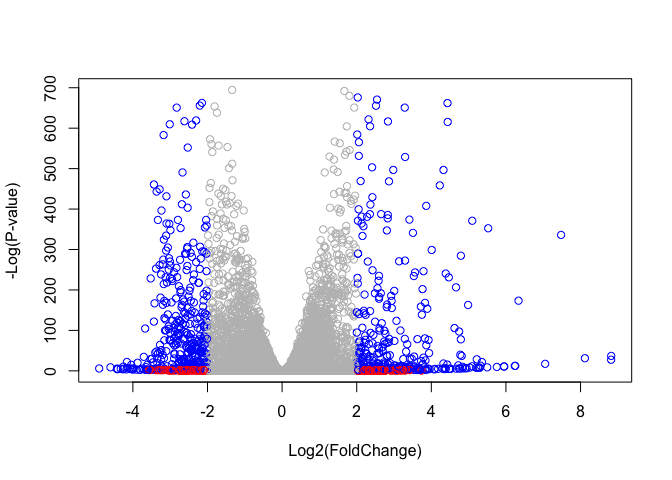
\includegraphics{test_files/figure-latex/unnamed-chunk-14-1.pdf}

The second plot is shifted down and there is more overlap between the
diagnosis. \#making ggplot:

\begin{Shaded}
\begin{Highlighting}[]
\CommentTok{\# Create a data.frame for ggplot}
\NormalTok{df }\OtherTok{\textless{}{-}} \FunctionTok{as.data.frame}\NormalTok{(wisc.pr}\SpecialCharTok{$}\NormalTok{x)}
\NormalTok{df}\SpecialCharTok{$}\NormalTok{diagnosis }\OtherTok{\textless{}{-}}\NormalTok{ diagnosis}

\CommentTok{\# Load the ggplot2 package}
\FunctionTok{library}\NormalTok{(ggplot2)}

\CommentTok{\# Make a scatter plot colored by diagnosis}
\FunctionTok{ggplot}\NormalTok{(df) }\SpecialCharTok{+} 
  \FunctionTok{aes}\NormalTok{(PC1, PC2, }\AttributeTok{col=}\NormalTok{diagnosis) }\SpecialCharTok{+} 
  \FunctionTok{geom\_point}\NormalTok{()}
\end{Highlighting}
\end{Shaded}

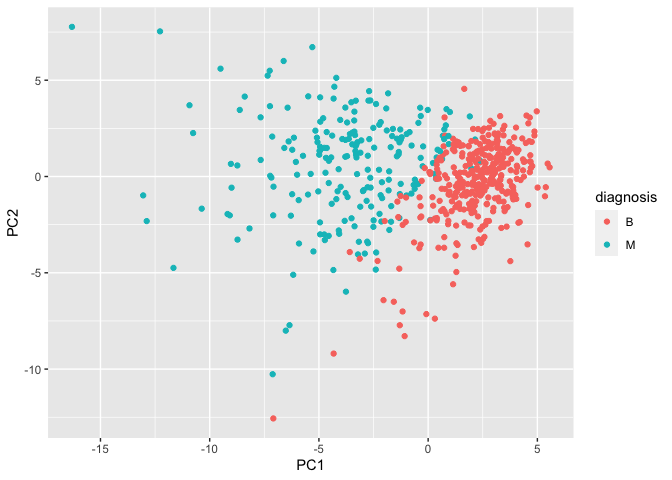
\includegraphics{test_files/figure-latex/unnamed-chunk-15-1.pdf}

\#Calculating variance

\begin{Shaded}
\begin{Highlighting}[]
\CommentTok{\# Calculate variance of each component}
\NormalTok{pr.var }\OtherTok{\textless{}{-}}\NormalTok{ wisc.pr}\SpecialCharTok{$}\NormalTok{sdev}\SpecialCharTok{\^{}}\DecValTok{2}
\FunctionTok{head}\NormalTok{(pr.var)}
\end{Highlighting}
\end{Shaded}

\begin{verbatim}
## [1] 13.281608  5.691355  2.817949  1.980640  1.648731  1.207357
\end{verbatim}

\begin{Shaded}
\begin{Highlighting}[]
\CommentTok{\# Variance explained by each principal component: pve}
\NormalTok{pve }\OtherTok{\textless{}{-}}\NormalTok{ pr.var }\SpecialCharTok{/} \FunctionTok{sum}\NormalTok{(pr.var)}

\CommentTok{\# Plot variance explained for each principal component}
\FunctionTok{plot}\NormalTok{(pve, }\AttributeTok{xlab =} \StringTok{"Principal Component"}\NormalTok{, }
     \AttributeTok{ylab =} \StringTok{"Proportion of Variance Explained"}\NormalTok{, }
     \AttributeTok{ylim =} \FunctionTok{c}\NormalTok{(}\DecValTok{0}\NormalTok{, }\DecValTok{1}\NormalTok{), }\AttributeTok{type =} \StringTok{"o"}\NormalTok{)}
\end{Highlighting}
\end{Shaded}

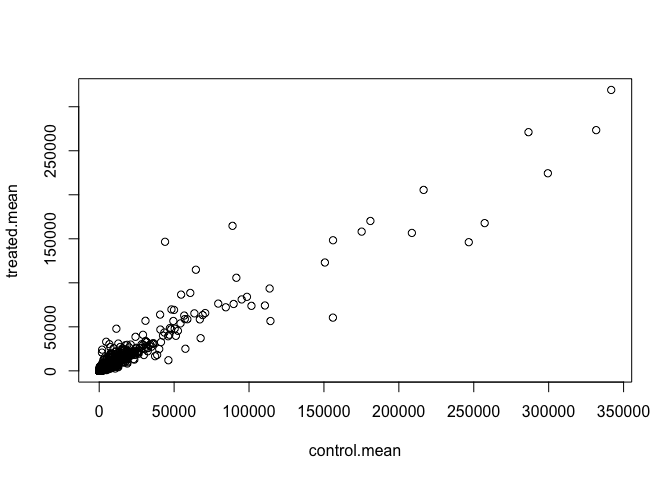
\includegraphics{test_files/figure-latex/unnamed-chunk-17-1.pdf}

\begin{Shaded}
\begin{Highlighting}[]
\CommentTok{\# Alternative scree plot of the same data, note data driven y{-}axis}
\FunctionTok{barplot}\NormalTok{(pve, }\AttributeTok{ylab =} \StringTok{"Precent of Variance Explained"}\NormalTok{,}
     \AttributeTok{names.arg=}\FunctionTok{paste0}\NormalTok{(}\StringTok{"PC"}\NormalTok{,}\DecValTok{1}\SpecialCharTok{:}\FunctionTok{length}\NormalTok{(pve)), }\AttributeTok{las=}\DecValTok{2}\NormalTok{, }\AttributeTok{axes =} \ConstantTok{FALSE}\NormalTok{)}
\FunctionTok{axis}\NormalTok{(}\DecValTok{2}\NormalTok{, }\AttributeTok{at=}\NormalTok{pve, }\AttributeTok{labels=}\FunctionTok{round}\NormalTok{(pve,}\DecValTok{2}\NormalTok{)}\SpecialCharTok{*}\DecValTok{100}\NormalTok{ )}
\end{Highlighting}
\end{Shaded}

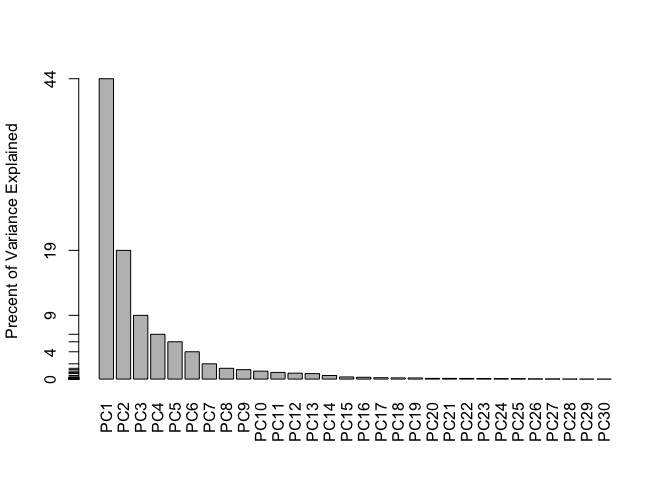
\includegraphics{test_files/figure-latex/unnamed-chunk-18-1.pdf}

\#Q9. For the first principal component, what is the component of the
loading vector (i.e.~wisc.pr\$rotation{[},1{]}) for the feature
concave.points\_mean?

\begin{Shaded}
\begin{Highlighting}[]
\NormalTok{wisc.pr}\SpecialCharTok{$}\NormalTok{rotation[,}\DecValTok{1}\NormalTok{]}
\end{Highlighting}
\end{Shaded}

\begin{verbatim}
##             radius_mean            texture_mean          perimeter_mean 
##             -0.21890244             -0.10372458             -0.22753729 
##               area_mean         smoothness_mean        compactness_mean 
##             -0.22099499             -0.14258969             -0.23928535 
##          concavity_mean     concave.points_mean           symmetry_mean 
##             -0.25840048             -0.26085376             -0.13816696 
##  fractal_dimension_mean               radius_se              texture_se 
##             -0.06436335             -0.20597878             -0.01742803 
##            perimeter_se                 area_se           smoothness_se 
##             -0.21132592             -0.20286964             -0.01453145 
##          compactness_se            concavity_se       concave.points_se 
##             -0.17039345             -0.15358979             -0.18341740 
##             symmetry_se    fractal_dimension_se            radius_worst 
##             -0.04249842             -0.10256832             -0.22799663 
##           texture_worst         perimeter_worst              area_worst 
##             -0.10446933             -0.23663968             -0.22487053 
##        smoothness_worst       compactness_worst         concavity_worst 
##             -0.12795256             -0.21009588             -0.22876753 
##    concave.points_worst          symmetry_worst fractal_dimension_worst 
##             -0.25088597             -0.12290456             -0.13178394
\end{verbatim}

The component of concave.points\_mean is -0.26085376.

\#Q10. What is the minimum number of principal components required to
explain 80\% of the variance of the data?

\begin{Shaded}
\begin{Highlighting}[]
\FunctionTok{summary}\NormalTok{(wisc.pr)}
\end{Highlighting}
\end{Shaded}

\begin{verbatim}
## Importance of components:
##                           PC1    PC2     PC3     PC4     PC5     PC6     PC7
## Standard deviation     3.6444 2.3857 1.67867 1.40735 1.28403 1.09880 0.82172
## Proportion of Variance 0.4427 0.1897 0.09393 0.06602 0.05496 0.04025 0.02251
## Cumulative Proportion  0.4427 0.6324 0.72636 0.79239 0.84734 0.88759 0.91010
##                            PC8    PC9    PC10   PC11    PC12    PC13    PC14
## Standard deviation     0.69037 0.6457 0.59219 0.5421 0.51104 0.49128 0.39624
## Proportion of Variance 0.01589 0.0139 0.01169 0.0098 0.00871 0.00805 0.00523
## Cumulative Proportion  0.92598 0.9399 0.95157 0.9614 0.97007 0.97812 0.98335
##                           PC15    PC16    PC17    PC18    PC19    PC20   PC21
## Standard deviation     0.30681 0.28260 0.24372 0.22939 0.22244 0.17652 0.1731
## Proportion of Variance 0.00314 0.00266 0.00198 0.00175 0.00165 0.00104 0.0010
## Cumulative Proportion  0.98649 0.98915 0.99113 0.99288 0.99453 0.99557 0.9966
##                           PC22    PC23   PC24    PC25    PC26    PC27    PC28
## Standard deviation     0.16565 0.15602 0.1344 0.12442 0.09043 0.08307 0.03987
## Proportion of Variance 0.00091 0.00081 0.0006 0.00052 0.00027 0.00023 0.00005
## Cumulative Proportion  0.99749 0.99830 0.9989 0.99942 0.99969 0.99992 0.99997
##                           PC29    PC30
## Standard deviation     0.02736 0.01153
## Proportion of Variance 0.00002 0.00000
## Cumulative Proportion  1.00000 1.00000
\end{verbatim}

You need 5 PCs to explain 80\% of the variance in the data.

\#\#Hierarchical clustering

\begin{Shaded}
\begin{Highlighting}[]
\CommentTok{\# Scale the wisc.data data using the "scale()" function}
\NormalTok{data.scaled }\OtherTok{\textless{}{-}} \FunctionTok{scale}\NormalTok{(wisc.data)}
\end{Highlighting}
\end{Shaded}

\begin{Shaded}
\begin{Highlighting}[]
\CommentTok{\#calculating elucidian data}
\NormalTok{data.dist }\OtherTok{\textless{}{-}} \FunctionTok{dist}\NormalTok{(data.scaled)}
\CommentTok{\#data.dist}
\end{Highlighting}
\end{Shaded}

\#Q11. Using the plot() and abline() functions, what is the height at
which the clustering model has 4 clusters?

\begin{Shaded}
\begin{Highlighting}[]
\NormalTok{wisc.hclust }\OtherTok{\textless{}{-}} \FunctionTok{hclust}\NormalTok{(data.dist, }\AttributeTok{method=} \StringTok{"complete"}\NormalTok{)}
\NormalTok{wisc.hclust}
\end{Highlighting}
\end{Shaded}

\begin{verbatim}
## 
## Call:
## hclust(d = data.dist, method = "complete")
## 
## Cluster method   : complete 
## Distance         : euclidean 
## Number of objects: 569
\end{verbatim}

\begin{Shaded}
\begin{Highlighting}[]
\FunctionTok{plot}\NormalTok{(wisc.hclust)}
\FunctionTok{abline}\NormalTok{(}\AttributeTok{h=}\DecValTok{19}\NormalTok{, }\AttributeTok{col=}\StringTok{"red"}\NormalTok{, }\AttributeTok{lty=}\DecValTok{2}\NormalTok{)}
\end{Highlighting}
\end{Shaded}

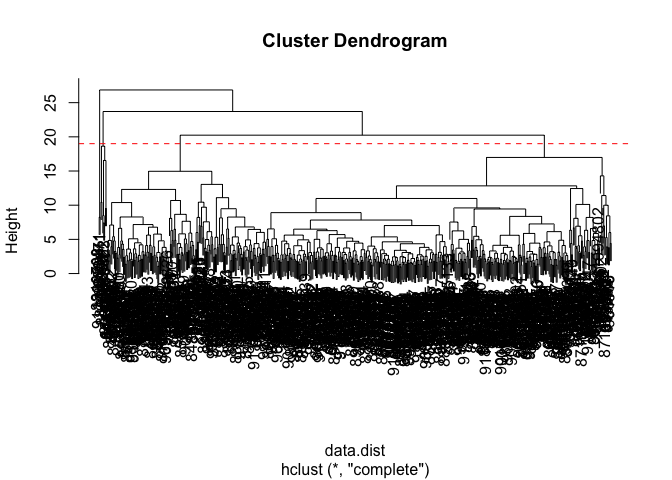
\includegraphics{test_files/figure-latex/unnamed-chunk-24-1.pdf}

The height at which there is 4 clusters is around 19.

\begin{Shaded}
\begin{Highlighting}[]
\NormalTok{wisc.hclust.clusters }\OtherTok{\textless{}{-}} \FunctionTok{cutree}\NormalTok{(wisc.hclust, }\DecValTok{4}\NormalTok{)}
\NormalTok{wisc.hclust.clusters}
\end{Highlighting}
\end{Shaded}

\begin{verbatim}
##    842302    842517  84300903  84348301  84358402    843786    844359  84458202 
##         1         1         1         2         1         1         1         1 
##    844981  84501001    845636  84610002    846226    846381  84667401  84799002 
##         1         2         3         1         1         3         1         1 
##    848406  84862001    849014   8510426   8510653   8510824   8511133    851509 
##         3         1         1         3         3         3         1         1 
##    852552    852631    852763    852781    852973    853201    853401    853612 
##         1         1         1         1         1         3         1         1 
##  85382601    854002    854039    854253    854268    854941    855133    855138 
##         1         1         1         1         1         3         3         1 
##    855167    855563    855625    856106  85638502    857010  85713702     85715 
##         3         1         1         1         1         1         3         1 
##    857155    857156    857343    857373    857374    857392    857438  85759902 
##         3         3         3         3         3         1         3         3 
##    857637    857793    857810    858477    858970    858981    858986    859196 
##         1         1         3         3         3         3         1         3 
##  85922302    859283    859464    859465    859471    859487    859575    859711 
##         1         1         3         3         2         3         1         3 
##    859717    859983   8610175   8610404   8610629   8610637   8610862   8610908 
##         1         1         3         3         3         1         2         3 
##    861103   8611161   8611555   8611792   8612080   8612399  86135501  86135502 
##         3         1         1         1         3         1         3         1 
##    861597    861598    861648    861799    861853    862009    862028     86208 
##         3         1         3         3         3         3         1         1 
##     86211    862261    862485    862548    862717    862722    862965    862980 
##         3         3         3         3         3         3         3         3 
##    862989    863030    863031    863270     86355    864018    864033     86408 
##         3         1         1         3         1         3         3         3 
##     86409    864292    864496    864685    864726    864729    864877    865128 
##         3         3         3         3         3         1         1         3 
##    865137     86517    865423    865432    865468     86561    866083    866203 
##         3         1         2         3         3         3         1         3 
##    866458    866674    866714      8670  86730502    867387    867739    868202 
##         1         1         3         1         1         3         1         3 
##    868223    868682    868826    868871    868999    869104    869218    869224 
##         3         3         1         3         3         3         3         3 
##    869254    869476    869691  86973701  86973702    869931 871001501 871001502 
##         3         3         1         3         3         3         3         3 
##   8710441     87106   8711002   8711003   8711202   8711216    871122    871149 
##         2         3         3         3         1         3         3         3 
##   8711561   8711803    871201   8712064   8712289   8712291     87127   8712729 
##         3         1         1         3         1         3         3         3 
##   8712766   8712853  87139402     87163     87164    871641    871642    872113 
##         1         3         3         3         1         3         3         3 
##    872608  87281702    873357    873586    873592    873593    873701    873843 
##         3         1         3         3         1         1         1         3 
##    873885    874158    874217    874373    874662    874839    874858    875093 
##         1         3         3         3         3         3         2         3 
##    875099    875263  87556202    875878    875938    877159    877486    877500 
##         3         1         1         3         1         3         1         1 
##    877501    877989    878796     87880     87930    879523    879804    879830 
##         3         3         1         1         3         3         3         3 
##   8810158   8810436 881046502   8810528   8810703 881094802   8810955   8810987 
##         1         3         1         3         4         3         1         1 
##   8811523   8811779   8811842  88119002   8812816   8812818   8812844   8812877 
##         3         3         1         1         3         3         3         1 
##   8813129  88143502  88147101  88147102  88147202    881861    881972  88199202 
##         3         3         3         3         3         1         1         3 
##  88203002  88206102    882488  88249602  88299702    883263    883270  88330202 
##         3         1         3         3         1         1         3         1 
##  88350402    883539    883852  88411702    884180    884437    884448    884626 
##         3         3         3         3         1         3         3         3 
##  88466802    884689    884948  88518501    885429   8860702    886226    886452 
##         3         3         1         3         1         3         1         3 
##  88649001    886776    887181  88725602    887549    888264    888570    889403 
##         1         1         1         1         1         3         1         3 
##    889719  88995002   8910251   8910499   8910506   8910720   8910721   8910748 
##         1         1         3         3         3         3         3         3 
##   8910988   8910996   8911163   8911164   8911230   8911670   8911800   8911834 
##         1         3         3         3         3         3         3         3 
##   8912049   8912055     89122   8912280   8912284   8912521   8912909      8913 
##         1         3         1         1         3         3         3         3 
##   8913049  89143601  89143602      8915    891670    891703    891716    891923 
##         3         3         3         3         3         3         3         3 
##    891936    892189    892214    892399    892438    892604  89263202    892657 
##         3         3         3         3         1         3         1         3 
##     89296    893061     89344     89346    893526    893548    893783  89382601 
##         3         3         3         3         3         3         3         3 
##  89382602    893988    894047    894089    894090    894326    894329    894335 
##         3         3         3         3         3         1         3         3 
##    894604    894618    894855    895100  89511501  89511502     89524    895299 
##         3         3         3         1         3         3         3         3 
##   8953902    895633    896839    896864    897132    897137    897374  89742801 
##         1         1         1         1         3         3         3         1 
##    897604    897630    897880     89812     89813    898143     89827    898431 
##         3         1         3         1         3         3         3         1 
##  89864002    898677    898678     89869    898690    899147    899187    899667 
##         3         3         3         3         3         3         3         1 
##    899987   9010018    901011   9010258   9010259    901028   9010333 901034301 
##         1         1         3         3         3         3         3         3 
## 901034302    901041   9010598   9010872   9010877    901088   9011494   9011495 
##         3         3         3         3         3         1         1         3 
##   9011971   9012000   9012315   9012568   9012795    901288   9013005    901303 
##         1         1         1         3         1         1         3         3 
##    901315   9013579   9013594   9013838    901549    901836     90250     90251 
##         3         3         3         1         3         3         3         3 
##    902727     90291    902975    902976    903011     90312  90317302    903483 
##         3         3         3         3         3         1         3         3 
##    903507    903516    903554    903811  90401601  90401602    904302    904357 
##         1         1         3         3         3         3         3         3 
##  90439701    904647    904689      9047    904969    904971    905189    905190 
##         1         3         3         3         3         3         3         3 
##  90524101    905501    905502    905520    905539    905557    905680    905686 
##         1         3         3         3         3         3         3         3 
##    905978  90602302    906024    906290    906539    906564    906616    906878 
##         3         1         3         3         3         1         3         3 
##    907145    907367    907409     90745  90769601  90769602    907914    907915 
##         3         3         3         3         3         3         1         3 
##    908194    908445    908469    908489    908916    909220    909231    909410 
##         1         1         3         1         3         3         3         3 
##    909411    909445  90944601    909777   9110127   9110720   9110732   9110944 
##         3         3         3         3         3         3         1         3 
##    911150 911157302   9111596   9111805   9111843    911201    911202   9112085 
##         3         1         3         1         3         3         3         3 
##   9112366   9112367   9112594   9112712 911296201 911296202   9113156 911320501 
##         3         3         3         3         1         4         3         3 
## 911320502   9113239   9113455   9113514   9113538    911366   9113778   9113816 
##         3         3         3         3         1         1         3         3 
##    911384   9113846    911391    911408    911654    911673    911685    911916 
##         3         3         3         3         3         3         3         1 
##    912193     91227    912519    912558    912600    913063    913102    913505 
##         3         3         3         3         3         3         3         1 
##    913512    913535  91376701  91376702    914062    914101    914102    914333 
##         3         3         3         3         1         3         3         3 
##    914366    914580    914769     91485    914862     91504     91505    915143 
##         1         3         1         1         3         1         3         1 
##    915186    915276  91544001  91544002    915452    915460     91550    915664 
##         3         3         3         3         3         1         3         3 
##    915691    915940  91594602    916221    916799    916838    917062    917080 
##         1         3         3         3         1         1         3         3 
##    917092  91762702     91789    917896    917897     91805  91813701  91813702 
##         3         1         3         3         3         3         1         3 
##    918192    918465     91858  91903901  91903902  91930402    919537    919555 
##         3         3         3         3         3         1         3         1 
##  91979701    919812    921092    921362    921385    921386    921644    922296 
##         3         1         3         3         3         1         3         3 
##    922297    922576    922577    922840    923169    923465    923748    923780 
##         3         3         3         3         3         3         3         3 
##    924084    924342    924632    924934    924964    925236    925277    925291 
##         3         3         3         3         3         3         3         3 
##    925292    925311    925622    926125    926424    926682    926954    927241 
##         3         3         1         1         1         1         3         1 
##     92751 
##         3
\end{verbatim}

\begin{Shaded}
\begin{Highlighting}[]
\FunctionTok{table}\NormalTok{(wisc.hclust.clusters, diagnosis)}
\end{Highlighting}
\end{Shaded}

\begin{verbatim}
##                     diagnosis
## wisc.hclust.clusters   B   M
##                    1  12 165
##                    2   2   5
##                    3 343  40
##                    4   0   2
\end{verbatim}

\#Q12. Can you find a better cluster vs diagnoses match by cutting into
a different number of clusters between 2 and 10?

\begin{Shaded}
\begin{Highlighting}[]
\NormalTok{wisc.hclust.clusters }\OtherTok{\textless{}{-}} \FunctionTok{cutree}\NormalTok{(wisc.hclust, }\DecValTok{4}\NormalTok{)}
\FunctionTok{table}\NormalTok{(wisc.hclust.clusters, diagnosis)}
\end{Highlighting}
\end{Shaded}

\begin{verbatim}
##                     diagnosis
## wisc.hclust.clusters   B   M
##                    1  12 165
##                    2   2   5
##                    3 343  40
##                    4   0   2
\end{verbatim}

We like 4 because that is where the diagnosis information really splits
off from each other.

\#Q13. Which method gives your favorite results for the same data.dist
dataset? Explain your reasoning.

\begin{Shaded}
\begin{Highlighting}[]
\NormalTok{wisc.hclust1 }\OtherTok{\textless{}{-}} \FunctionTok{hclust}\NormalTok{(data.dist, }\AttributeTok{method=} \StringTok{"ward.D2"}\NormalTok{)}
\NormalTok{wisc.hclust1}
\end{Highlighting}
\end{Shaded}

\begin{verbatim}
## 
## Call:
## hclust(d = data.dist, method = "ward.D2")
## 
## Cluster method   : ward.D2 
## Distance         : euclidean 
## Number of objects: 569
\end{verbatim}

\begin{Shaded}
\begin{Highlighting}[]
\FunctionTok{plot}\NormalTok{(wisc.hclust1)}
\FunctionTok{abline}\NormalTok{(}\AttributeTok{h=}\DecValTok{80}\NormalTok{, }\AttributeTok{col=}\StringTok{\textquotesingle{}red\textquotesingle{}}\NormalTok{)}
\end{Highlighting}
\end{Shaded}

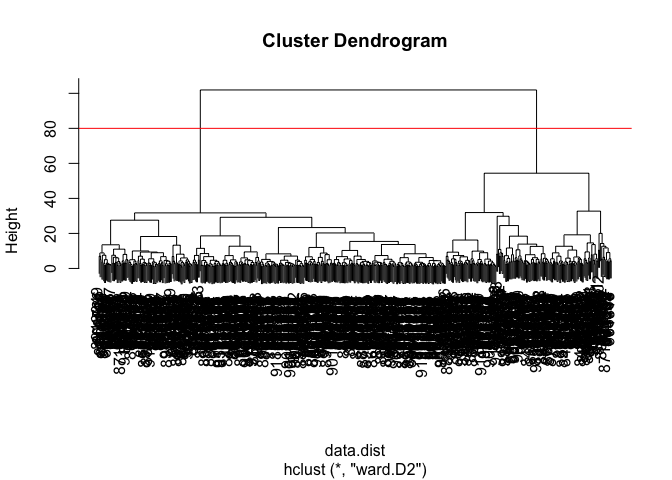
\includegraphics{test_files/figure-latex/unnamed-chunk-28-1.pdf} We like
ward.D2 because it splits it into two separate clusters initially.

Attempt at individually coding the below:

\begin{Shaded}
\begin{Highlighting}[]
\NormalTok{data.scaled}\FloatTok{.90} \OtherTok{\textless{}{-}} \FunctionTok{scale}\NormalTok{(wisc.data[,}\DecValTok{1}\SpecialCharTok{:}\DecValTok{7}\NormalTok{])}
\NormalTok{data.dist}\FloatTok{.90} \OtherTok{\textless{}{-}} \FunctionTok{dist}\NormalTok{(data.scaled}\FloatTok{.90}\NormalTok{)}
\NormalTok{wisc.pr.hclust1 }\OtherTok{\textless{}{-}} \FunctionTok{hclust}\NormalTok{(data.dist}\FloatTok{.90}\NormalTok{, }\AttributeTok{method=} \StringTok{"ward.D2"}\NormalTok{)}
\NormalTok{wisc.pr.hclust1}
\end{Highlighting}
\end{Shaded}

\begin{verbatim}
## 
## Call:
## hclust(d = data.dist.90, method = "ward.D2")
## 
## Cluster method   : ward.D2 
## Distance         : euclidean 
## Number of objects: 569
\end{verbatim}

\begin{Shaded}
\begin{Highlighting}[]
\FunctionTok{plot}\NormalTok{(wisc.pr.hclust1)}
\end{Highlighting}
\end{Shaded}

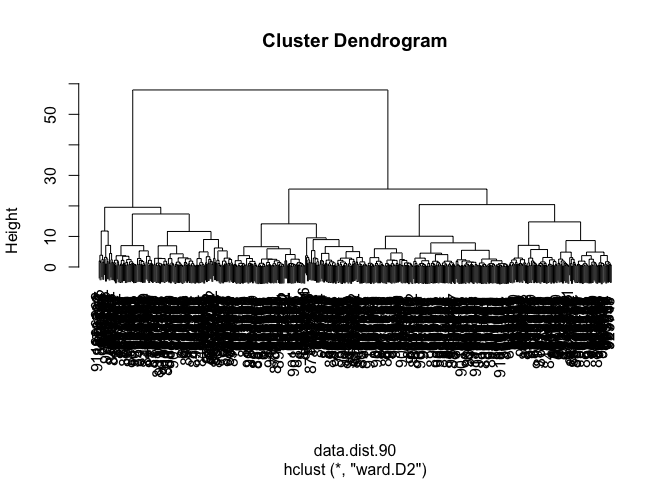
\includegraphics{test_files/figure-latex/unnamed-chunk-29-1.pdf}

CLuster my PCA results I will use 7 PCs and \texttt{hclust} and
\texttt{dist()} as an input

\begin{Shaded}
\begin{Highlighting}[]
\NormalTok{wisc.pr.hclust }\OtherTok{\textless{}{-}}\FunctionTok{hclust}\NormalTok{(}\FunctionTok{dist}\NormalTok{(wisc.pr}\SpecialCharTok{$}\NormalTok{x[,}\DecValTok{1}\SpecialCharTok{:}\DecValTok{7}\NormalTok{]), }\AttributeTok{method=}\StringTok{"ward.D2"}\NormalTok{)}
\NormalTok{wisc.pr.hclust}
\end{Highlighting}
\end{Shaded}

\begin{verbatim}
## 
## Call:
## hclust(d = dist(wisc.pr$x[, 1:7]), method = "ward.D2")
## 
## Cluster method   : ward.D2 
## Distance         : euclidean 
## Number of objects: 569
\end{verbatim}

\begin{Shaded}
\begin{Highlighting}[]
\FunctionTok{plot}\NormalTok{(wisc.pr.hclust)}
\FunctionTok{abline}\NormalTok{(}\AttributeTok{h=}\DecValTok{80}\NormalTok{, }\AttributeTok{col=}\StringTok{\textquotesingle{}red\textquotesingle{}}\NormalTok{)}
\end{Highlighting}
\end{Shaded}

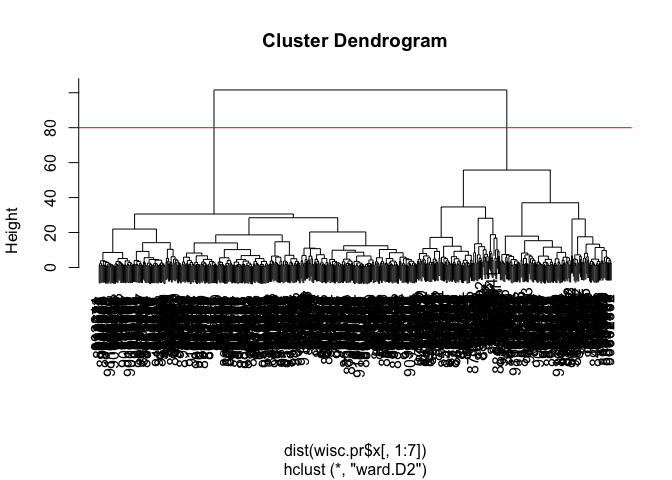
\includegraphics{test_files/figure-latex/unnamed-chunk-30-1.pdf}

Lets fnd our cluster memebership vecotr by cutting this tree into k=2
groups

\begin{Shaded}
\begin{Highlighting}[]
\NormalTok{grps }\OtherTok{\textless{}{-}}\FunctionTok{cutree}\NormalTok{(wisc.pr.hclust, }\AttributeTok{k=}\DecValTok{2}\NormalTok{)}
\FunctionTok{table}\NormalTok{(grps)}
\end{Highlighting}
\end{Shaded}

\begin{verbatim}
## grps
##   1   2 
## 216 353
\end{verbatim}

We can do a cross table by giving the \texttt{table()} two inputs. We
get True positives:188, False positives: 28, True negatives: 329, and
false negatives: 24

\begin{Shaded}
\begin{Highlighting}[]
\FunctionTok{table}\NormalTok{(grps, diagnosis)}
\end{Highlighting}
\end{Shaded}

\begin{verbatim}
##     diagnosis
## grps   B   M
##    1  28 188
##    2 329  24
\end{verbatim}

\textbf{Accuracy}, essentially how many did we get correct?

\begin{Shaded}
\begin{Highlighting}[]
\NormalTok{(}\DecValTok{188}\SpecialCharTok{+}\DecValTok{329}\NormalTok{)}\SpecialCharTok{/}\FunctionTok{nrow}\NormalTok{(wisc.data)}
\end{Highlighting}
\end{Shaded}

\begin{verbatim}
## [1] 0.9086116
\end{verbatim}

Sensitivity/Specificity: sensitivity refers to tests ability to
correctly detect ill patients who do have the condition. In our example
here the sensitivity is the total number of samples in the cluster
identified as predominantly malignant (cancerous) divided by the total
number of known malignant samples. In other words: TP/(TP+FN).

\begin{Shaded}
\begin{Highlighting}[]
\DecValTok{188}\SpecialCharTok{/}\NormalTok{(}\DecValTok{188}\SpecialCharTok{+}\DecValTok{24}\NormalTok{)}
\end{Highlighting}
\end{Shaded}

\begin{verbatim}
## [1] 0.8867925
\end{verbatim}

Specificity relates to a test's ability to correctly reject healthy
patients without a condition. In our example specificity is the
proportion of benign (not cancerous) samples in the cluster identified
as predominantly benign that are known to be benign. In other words:
TN/(TN+FN).

\begin{Shaded}
\begin{Highlighting}[]
\DecValTok{329}\SpecialCharTok{/}\NormalTok{(}\DecValTok{329}\SpecialCharTok{+}\DecValTok{24}\NormalTok{)}
\end{Highlighting}
\end{Shaded}

\begin{verbatim}
## [1] 0.9320113
\end{verbatim}

We would want to increase the sensitivity as much as possible because it
would be better to say a healthy patient is sick than a sick patient is
healthy. That would be limited if we increased the sensitivity.

\#7: Predictions

\begin{Shaded}
\begin{Highlighting}[]
\NormalTok{url }\OtherTok{\textless{}{-}} \StringTok{"new\_samples.csv"}
\NormalTok{url }\OtherTok{\textless{}{-}} \StringTok{"https://tinyurl.com/new{-}samples{-}CSV"}
\NormalTok{new }\OtherTok{\textless{}{-}} \FunctionTok{read.csv}\NormalTok{(url)}
\NormalTok{npc }\OtherTok{\textless{}{-}} \FunctionTok{predict}\NormalTok{(wisc.pr, }\AttributeTok{newdata=}\NormalTok{new)}
\NormalTok{npc}
\end{Highlighting}
\end{Shaded}

\begin{verbatim}
##            PC1        PC2        PC3       PC4      PC5       PC6        PC7
## [1,] -10.76452 -10.093978 -0.5897994 -4.164748 10.61922 -1.630738 0.03566861
## [2,] -18.09606  -9.967098 -2.1549431 -4.006848  6.69687 -2.034714 1.25088149
##            PC8       PC9     PC10       PC11     PC12       PC13      PC14
## [1,] 0.7308658 -1.580861 3.166451 -0.7167150 3.850569 -0.8259764 1.0195729
## [2,] 0.6308585 -1.155629 3.608207 -0.3405375 2.288732 -0.3976672 0.1347203
##          PC15      PC16      PC17      PC18     PC19      PC20      PC21
## [1,] 3.735687 -4.068783 1.0877034 0.9985959 1.022760 -2.430215 -1.295749
## [2,] 3.543905 -3.749616 0.7613603 1.1763217 1.366702 -2.609643 -1.541050
##           PC22       PC23      PC24       PC25      PC26      PC27       PC28
## [1,] -1.348026 -0.7388274 -1.083000 -0.4220831 -1.892993 -1.176056 0.05527974
## [2,] -1.424290 -0.7591376 -1.439202 -0.6508838 -1.981711 -1.397390 0.18112357
##           PC29       PC30
## [1,] 0.2658028 0.05162840
## [2,] 0.2842191 0.02734355
\end{verbatim}

plotting:

\begin{Shaded}
\begin{Highlighting}[]
\FunctionTok{plot}\NormalTok{(wisc.pr}\SpecialCharTok{$}\NormalTok{x[,}\DecValTok{1}\SpecialCharTok{:}\DecValTok{2}\NormalTok{], }\AttributeTok{col=}\NormalTok{diagnosis)}
\FunctionTok{points}\NormalTok{(npc[,}\DecValTok{1}\NormalTok{], npc[,}\DecValTok{2}\NormalTok{], }\AttributeTok{col=}\StringTok{"blue"}\NormalTok{, }\AttributeTok{pch=}\DecValTok{16}\NormalTok{, }\AttributeTok{cex=}\DecValTok{3}\NormalTok{)}
\FunctionTok{text}\NormalTok{(npc[,}\DecValTok{1}\NormalTok{], npc[,}\DecValTok{2}\NormalTok{], }\FunctionTok{c}\NormalTok{(}\DecValTok{1}\NormalTok{,}\DecValTok{2}\NormalTok{), }\AttributeTok{col=}\StringTok{"white"}\NormalTok{)}
\end{Highlighting}
\end{Shaded}

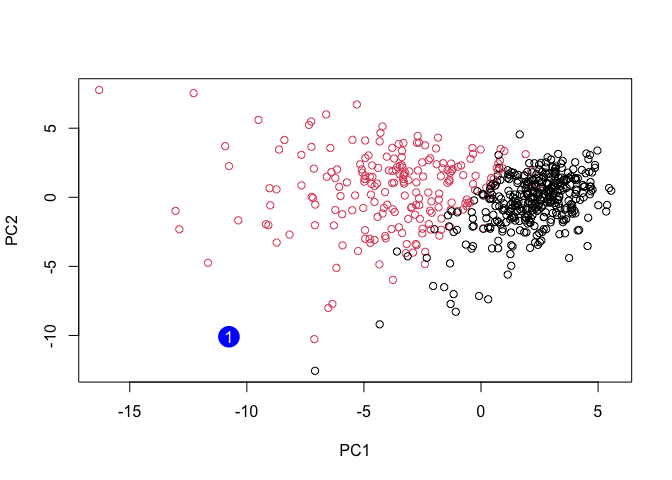
\includegraphics{test_files/figure-latex/unnamed-chunk-37-1.pdf}

Part 5 continued:

\begin{Shaded}
\begin{Highlighting}[]
\FunctionTok{plot}\NormalTok{(wisc.pr}\SpecialCharTok{$}\NormalTok{x[,}\DecValTok{1}\SpecialCharTok{:}\DecValTok{2}\NormalTok{], }\AttributeTok{col=}\NormalTok{grps)}
\end{Highlighting}
\end{Shaded}

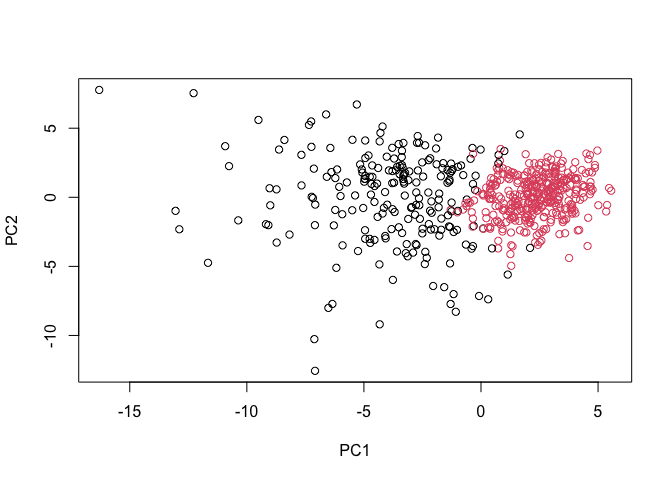
\includegraphics{test_files/figure-latex/unnamed-chunk-38-1.pdf}

\begin{Shaded}
\begin{Highlighting}[]
\FunctionTok{plot}\NormalTok{(wisc.pr}\SpecialCharTok{$}\NormalTok{x[,}\DecValTok{1}\SpecialCharTok{:}\DecValTok{2}\NormalTok{], }\AttributeTok{col=}\NormalTok{diagnosis)}
\end{Highlighting}
\end{Shaded}

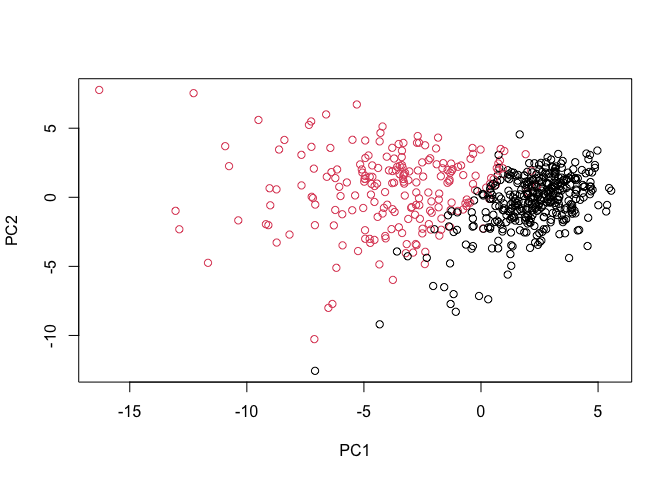
\includegraphics{test_files/figure-latex/unnamed-chunk-39-1.pdf}

\#Halloween Candy Project:

\begin{Shaded}
\begin{Highlighting}[]
\NormalTok{candy}\OtherTok{=}\FunctionTok{read.csv}\NormalTok{(}\StringTok{"https://raw.githubusercontent.com/fivethirtyeight/data/master/candy{-}power{-}ranking/candy{-}data.csv"}\NormalTok{, }\AttributeTok{row.names=}\DecValTok{1}\NormalTok{)}

\NormalTok{candy\_file}\OtherTok{\textless{}{-}}\StringTok{"https://raw.githubusercontent.com/fivethirtyeight/data/master/candy{-}power{-}ranking/candy{-}data.csv"}

\FunctionTok{head}\NormalTok{(candy)}
\end{Highlighting}
\end{Shaded}

\begin{verbatim}
##              chocolate fruity caramel peanutyalmondy nougat crispedricewafer
## 100 Grand            1      0       1              0      0                1
## 3 Musketeers         1      0       0              0      1                0
## One dime             0      0       0              0      0                0
## One quarter          0      0       0              0      0                0
## Air Heads            0      1       0              0      0                0
## Almond Joy           1      0       0              1      0                0
##              hard bar pluribus sugarpercent pricepercent winpercent
## 100 Grand       0   1        0        0.732        0.860   66.97173
## 3 Musketeers    0   1        0        0.604        0.511   67.60294
## One dime        0   0        0        0.011        0.116   32.26109
## One quarter     0   0        0        0.011        0.511   46.11650
## Air Heads       0   0        0        0.906        0.511   52.34146
## Almond Joy      0   1        0        0.465        0.767   50.34755
\end{verbatim}

\begin{Shaded}
\begin{Highlighting}[]
\FunctionTok{head}\NormalTok{(candy)}
\end{Highlighting}
\end{Shaded}

\begin{verbatim}
##              chocolate fruity caramel peanutyalmondy nougat crispedricewafer
## 100 Grand            1      0       1              0      0                1
## 3 Musketeers         1      0       0              0      1                0
## One dime             0      0       0              0      0                0
## One quarter          0      0       0              0      0                0
## Air Heads            0      1       0              0      0                0
## Almond Joy           1      0       0              1      0                0
##              hard bar pluribus sugarpercent pricepercent winpercent
## 100 Grand       0   1        0        0.732        0.860   66.97173
## 3 Musketeers    0   1        0        0.604        0.511   67.60294
## One dime        0   0        0        0.011        0.116   32.26109
## One quarter     0   0        0        0.011        0.511   46.11650
## Air Heads       0   0        0        0.906        0.511   52.34146
## Almond Joy      0   1        0        0.465        0.767   50.34755
\end{verbatim}

Q1. How many different candy types are in this dataset?

\begin{Shaded}
\begin{Highlighting}[]
\FunctionTok{nrow}\NormalTok{(candy)}
\end{Highlighting}
\end{Shaded}

\begin{verbatim}
## [1] 85
\end{verbatim}

Q2. How many fruity candy types are in the dataset?

\begin{Shaded}
\begin{Highlighting}[]
\FunctionTok{rownames}\NormalTok{(candy)}
\end{Highlighting}
\end{Shaded}

\begin{verbatim}
##  [1] "100 Grand"                   "3 Musketeers"               
##  [3] "One dime"                    "One quarter"                
##  [5] "Air Heads"                   "Almond Joy"                 
##  [7] "Baby Ruth"                   "Boston Baked Beans"         
##  [9] "Candy Corn"                  "Caramel Apple Pops"         
## [11] "Charleston Chew"             "Chewey Lemonhead Fruit Mix" 
## [13] "Chiclets"                    "Dots"                       
## [15] "Dum Dums"                    "Fruit Chews"                
## [17] "Fun Dip"                     "Gobstopper"                 
## [19] "Haribo Gold Bears"           "Haribo Happy Cola"          
## [21] "Haribo Sour Bears"           "Haribo Twin Snakes"         
## [23] "HersheyÕs Kisses"            "HersheyÕs Krackel"          
## [25] "HersheyÕs Milk Chocolate"    "HersheyÕs Special Dark"     
## [27] "Jawbusters"                  "Junior Mints"               
## [29] "Kit Kat"                     "Laffy Taffy"                
## [31] "Lemonhead"                   "Lifesavers big ring gummies"
## [33] "Peanut butter M&MÕs"         "M&MÕs"                      
## [35] "Mike & Ike"                  "Milk Duds"                  
## [37] "Milky Way"                   "Milky Way Midnight"         
## [39] "Milky Way Simply Caramel"    "Mounds"                     
## [41] "Mr Good Bar"                 "Nerds"                      
## [43] "Nestle Butterfinger"         "Nestle Crunch"              
## [45] "Nik L Nip"                   "Now & Later"                
## [47] "Payday"                      "Peanut M&Ms"                
## [49] "Pixie Sticks"                "Pop Rocks"                  
## [51] "Red vines"                   "ReeseÕs Miniatures"         
## [53] "ReeseÕs Peanut Butter cup"   "ReeseÕs pieces"             
## [55] "ReeseÕs stuffed with pieces" "Ring pop"                   
## [57] "Rolo"                        "Root Beer Barrels"          
## [59] "Runts"                       "Sixlets"                    
## [61] "Skittles original"           "Skittles wildberry"         
## [63] "Nestle Smarties"             "Smarties candy"             
## [65] "Snickers"                    "Snickers Crisper"           
## [67] "Sour Patch Kids"             "Sour Patch Tricksters"      
## [69] "Starburst"                   "Strawberry bon bons"        
## [71] "Sugar Babies"                "Sugar Daddy"                
## [73] "Super Bubble"                "Swedish Fish"               
## [75] "Tootsie Pop"                 "Tootsie Roll Juniors"       
## [77] "Tootsie Roll Midgies"        "Tootsie Roll Snack Bars"    
## [79] "Trolli Sour Bites"           "Twix"                       
## [81] "Twizzlers"                   "Warheads"                   
## [83] "WelchÕs Fruit Snacks"        "WertherÕs Original Caramel" 
## [85] "Whoppers"
\end{verbatim}

\begin{Shaded}
\begin{Highlighting}[]
\FunctionTok{rownames}\NormalTok{(candy)}\OtherTok{\textless{}{-}}\FunctionTok{gsub}\NormalTok{(}\StringTok{"Õ"}\NormalTok{,}\StringTok{"\textquotesingle{}"}\NormalTok{, }\FunctionTok{rownames}\NormalTok{(candy))}
\end{Highlighting}
\end{Shaded}

\begin{Shaded}
\begin{Highlighting}[]
\FunctionTok{sum}\NormalTok{(candy}\SpecialCharTok{$}\NormalTok{fruity)}
\end{Highlighting}
\end{Shaded}

\begin{verbatim}
## [1] 38
\end{verbatim}

\begin{Shaded}
\begin{Highlighting}[]
\NormalTok{candy[}\StringTok{"Twix"}\NormalTok{,]}\SpecialCharTok{$}\NormalTok{winpercent}
\end{Highlighting}
\end{Shaded}

\begin{verbatim}
## [1] 81.64291
\end{verbatim}

Q3. What is your favorite candy in the dataset and what is it's
winpercent value? Twix actually is my favorite candy, so its winpercent
is 81.64291

Q4. What is the winpercent value for ``Kit Kat''?

\begin{Shaded}
\begin{Highlighting}[]
\NormalTok{candy[}\StringTok{"Kit Kat"}\NormalTok{,]}\SpecialCharTok{$}\NormalTok{winpercent}
\end{Highlighting}
\end{Shaded}

\begin{verbatim}
## [1] 76.7686
\end{verbatim}

Q5. What is the winpercent value for ``Tootsie Roll Snack Bars''?

\begin{Shaded}
\begin{Highlighting}[]
\NormalTok{candy[}\StringTok{"Tootsie Roll Snack Bars"}\NormalTok{,]}\SpecialCharTok{$}\NormalTok{winpercent}
\end{Highlighting}
\end{Shaded}

\begin{verbatim}
## [1] 49.6535
\end{verbatim}

\begin{Shaded}
\begin{Highlighting}[]
\CommentTok{\#install.packages("skimr")}
\FunctionTok{library}\NormalTok{(}\StringTok{"skimr"}\NormalTok{)}
\FunctionTok{skim}\NormalTok{(candy)}
\end{Highlighting}
\end{Shaded}

\begin{longtable}[]{@{}ll@{}}
\caption{Data summary}\tabularnewline
\toprule
\endhead
Name & candy \\
Number of rows & 85 \\
Number of columns & 12 \\
\_\_\_\_\_\_\_\_\_\_\_\_\_\_\_\_\_\_\_\_\_\_\_ & \\
Column type frequency: & \\
numeric & 12 \\
\_\_\_\_\_\_\_\_\_\_\_\_\_\_\_\_\_\_\_\_\_\_\_\_ & \\
Group variables & None \\
\bottomrule
\end{longtable}

\textbf{Variable type: numeric}

\begin{longtable}[]{@{}lrrrrrrrrrl@{}}
\toprule
skim\_variable & n\_missing & complete\_rate & mean & sd & p0 & p25 &
p50 & p75 & p100 & hist \\
\midrule
\endhead
chocolate & 0 & 1 & 0.44 & 0.50 & 0.00 & 0.00 & 0.00 & 1.00 & 1.00 &
▇▁▁▁▆ \\
fruity & 0 & 1 & 0.45 & 0.50 & 0.00 & 0.00 & 0.00 & 1.00 & 1.00 &
▇▁▁▁▆ \\
caramel & 0 & 1 & 0.16 & 0.37 & 0.00 & 0.00 & 0.00 & 0.00 & 1.00 &
▇▁▁▁▂ \\
peanutyalmondy & 0 & 1 & 0.16 & 0.37 & 0.00 & 0.00 & 0.00 & 0.00 & 1.00
& ▇▁▁▁▂ \\
nougat & 0 & 1 & 0.08 & 0.28 & 0.00 & 0.00 & 0.00 & 0.00 & 1.00 &
▇▁▁▁▁ \\
crispedricewafer & 0 & 1 & 0.08 & 0.28 & 0.00 & 0.00 & 0.00 & 0.00 &
1.00 & ▇▁▁▁▁ \\
hard & 0 & 1 & 0.18 & 0.38 & 0.00 & 0.00 & 0.00 & 0.00 & 1.00 & ▇▁▁▁▂ \\
bar & 0 & 1 & 0.25 & 0.43 & 0.00 & 0.00 & 0.00 & 0.00 & 1.00 & ▇▁▁▁▂ \\
pluribus & 0 & 1 & 0.52 & 0.50 & 0.00 & 0.00 & 1.00 & 1.00 & 1.00 &
▇▁▁▁▇ \\
sugarpercent & 0 & 1 & 0.48 & 0.28 & 0.01 & 0.22 & 0.47 & 0.73 & 0.99 &
▇▇▇▇▆ \\
pricepercent & 0 & 1 & 0.47 & 0.29 & 0.01 & 0.26 & 0.47 & 0.65 & 0.98 &
▇▇▇▇▆ \\
winpercent & 0 & 1 & 50.32 & 14.71 & 22.45 & 39.14 & 47.83 & 59.86 &
84.18 & ▃▇▆▅▂ \\
\bottomrule
\end{longtable}

\#Q6. Is there any variable/column that looks to be on a different scale
to the majority of the other columns in the dataset? The last three rows
are percentage, and row 12 is multiplied by 100.

\#Q7. What do you think a zero and one represent for the
candy\$chocolate column? yes or no.

\#Q8. Plot a histogram of winpercent values

\begin{Shaded}
\begin{Highlighting}[]
\FunctionTok{hist}\NormalTok{(candy}\SpecialCharTok{$}\NormalTok{winpercent)}
\end{Highlighting}
\end{Shaded}

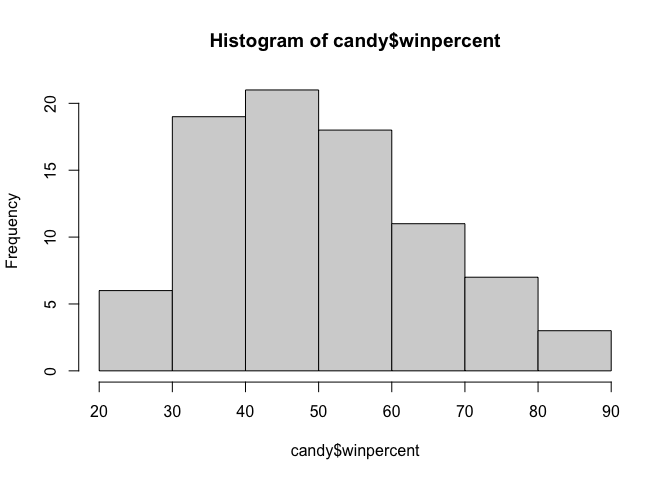
\includegraphics{test_files/figure-latex/unnamed-chunk-48-1.pdf}

\#Q9. Is the distribution of winpercent values symmetrical? No.~It is
shifted to 40 ish percent with few at 90. \#Q10. Is the center of the
distribution above or below 50\%? Below 50. \#Q11. On average is
chocolate candy higher or lower ranked than fruit candy?

\begin{Shaded}
\begin{Highlighting}[]
\NormalTok{chocolate }\OtherTok{\textless{}{-}}\NormalTok{ candy[}\FunctionTok{as.logical}\NormalTok{(candy}\SpecialCharTok{$}\NormalTok{chocolate),]}\SpecialCharTok{$}\NormalTok{winpercent}
\FunctionTok{mean}\NormalTok{(chocolate)}
\end{Highlighting}
\end{Shaded}

\begin{verbatim}
## [1] 60.92153
\end{verbatim}

\begin{Shaded}
\begin{Highlighting}[]
\NormalTok{fruity }\OtherTok{\textless{}{-}}\NormalTok{ candy[}\FunctionTok{as.logical}\NormalTok{(candy}\SpecialCharTok{$}\NormalTok{fruity),]}\SpecialCharTok{$}\NormalTok{winpercent}
\FunctionTok{mean}\NormalTok{(fruity)}
\end{Highlighting}
\end{Shaded}

\begin{verbatim}
## [1] 44.11974
\end{verbatim}

chocolate candy is higher ranked than fruity. \#Q12. Is this difference
statistically significant?

\begin{Shaded}
\begin{Highlighting}[]
\FunctionTok{t.test}\NormalTok{(chocolate, fruity)}
\end{Highlighting}
\end{Shaded}

\begin{verbatim}
## 
##  Welch Two Sample t-test
## 
## data:  chocolate and fruity
## t = 6.2582, df = 68.882, p-value = 2.871e-08
## alternative hypothesis: true difference in means is not equal to 0
## 95 percent confidence interval:
##  11.44563 22.15795
## sample estimates:
## mean of x mean of y 
##  60.92153  44.11974
\end{verbatim}

It is significant.

\#Q13. What are the five least liked candy types in this set?

\begin{Shaded}
\begin{Highlighting}[]
\CommentTok{\#head(candy[order(candy$winpercent),], n=5)}
\end{Highlighting}
\end{Shaded}

\#Q14. What are the top 5 all time favorite candy types out of this set?

\begin{Shaded}
\begin{Highlighting}[]
\CommentTok{\#head(candy[order(candy$winpercent, decreasing=TRUE),], n=5)}
\end{Highlighting}
\end{Shaded}

\#Q15. Make a first barplot of candy ranking based on winpercent values.
HINT: Use the aes(winpercent, rownames(candy)) for your first ggplot
like so:

\begin{Shaded}
\begin{Highlighting}[]
\CommentTok{\#library(ggplot2)}

\CommentTok{\#ggplot(candy) + }
  \FunctionTok{aes}\NormalTok{(winpercent, }\FunctionTok{rownames}\NormalTok{(candy)) }\SpecialCharTok{+}
  \FunctionTok{geom\_col}\NormalTok{()}
\end{Highlighting}
\end{Shaded}

\begin{verbatim}
## NULL
\end{verbatim}

Q16. This is quite ugly, use the reorder() function to get the bars
sorted by winpercent?

\begin{Shaded}
\begin{Highlighting}[]
\FunctionTok{ggplot}\NormalTok{(candy) }\SpecialCharTok{+} 
\FunctionTok{aes}\NormalTok{(winpercent, }\FunctionTok{reorder}\NormalTok{(}\FunctionTok{rownames}\NormalTok{(candy),winpercent)) }\SpecialCharTok{+}
  \FunctionTok{geom\_col}\NormalTok{()}
\end{Highlighting}
\end{Shaded}

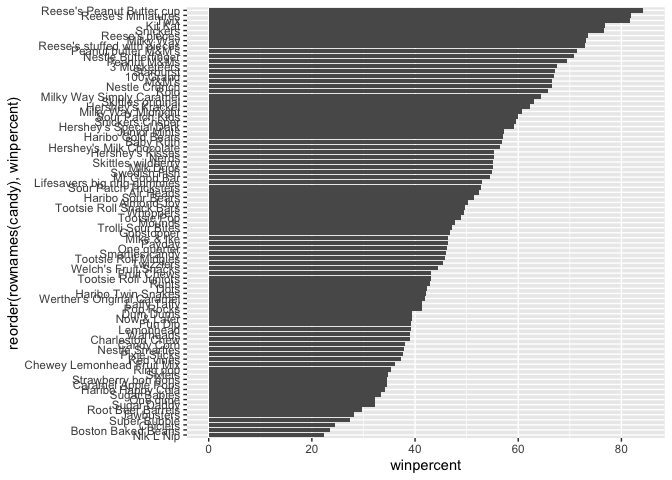
\includegraphics{test_files/figure-latex/unnamed-chunk-54-1.pdf} Making
colors

\begin{Shaded}
\begin{Highlighting}[]
\NormalTok{my\_cols}\OtherTok{=}\FunctionTok{rep}\NormalTok{(}\StringTok{"black"}\NormalTok{, }\FunctionTok{nrow}\NormalTok{(candy))}
\NormalTok{my\_cols[}\FunctionTok{as.logical}\NormalTok{(candy}\SpecialCharTok{$}\NormalTok{chocolate)] }\OtherTok{=} \StringTok{"chocolate"}
\NormalTok{my\_cols[}\FunctionTok{as.logical}\NormalTok{(candy}\SpecialCharTok{$}\NormalTok{bar)] }\OtherTok{=} \StringTok{"brown"}
\NormalTok{my\_cols[}\FunctionTok{as.logical}\NormalTok{(candy}\SpecialCharTok{$}\NormalTok{fruity)] }\OtherTok{=} \StringTok{"pink"}
\end{Highlighting}
\end{Shaded}

\begin{Shaded}
\begin{Highlighting}[]
\FunctionTok{ggplot}\NormalTok{(candy) }\SpecialCharTok{+} 
\FunctionTok{aes}\NormalTok{(winpercent, }\FunctionTok{reorder}\NormalTok{(}\FunctionTok{rownames}\NormalTok{(candy),winpercent)) }\SpecialCharTok{+}
  \FunctionTok{geom\_col}\NormalTok{(}\AttributeTok{fill=}\NormalTok{my\_cols)}
\end{Highlighting}
\end{Shaded}

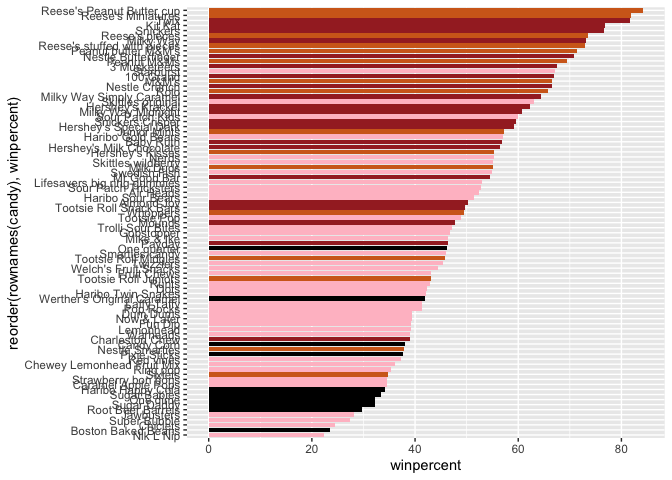
\includegraphics{test_files/figure-latex/unnamed-chunk-56-1.pdf} - Q17.
What is the worst ranked chocolate candy? The worst is Sixlets - Q18.
What is the best ranked fruity candy? The best fruity candy is
Starbursts

\begin{Shaded}
\begin{Highlighting}[]
\CommentTok{\#install.packages("ggrepel")}
\FunctionTok{library}\NormalTok{(ggrepel)}

\CommentTok{\# How about a plot of price vs win}
\FunctionTok{ggplot}\NormalTok{(candy) }\SpecialCharTok{+}
  \FunctionTok{aes}\NormalTok{(winpercent, pricepercent, }\AttributeTok{label=}\FunctionTok{rownames}\NormalTok{(candy)) }\SpecialCharTok{+}
  \FunctionTok{geom\_point}\NormalTok{(}\AttributeTok{col=}\NormalTok{my\_cols) }\SpecialCharTok{+} 
  \FunctionTok{geom\_text\_repel}\NormalTok{(}\AttributeTok{col=}\NormalTok{my\_cols, }\AttributeTok{size=}\FloatTok{3.3}\NormalTok{, }\AttributeTok{max.overlaps =} \DecValTok{20}\NormalTok{)}
\end{Highlighting}
\end{Shaded}

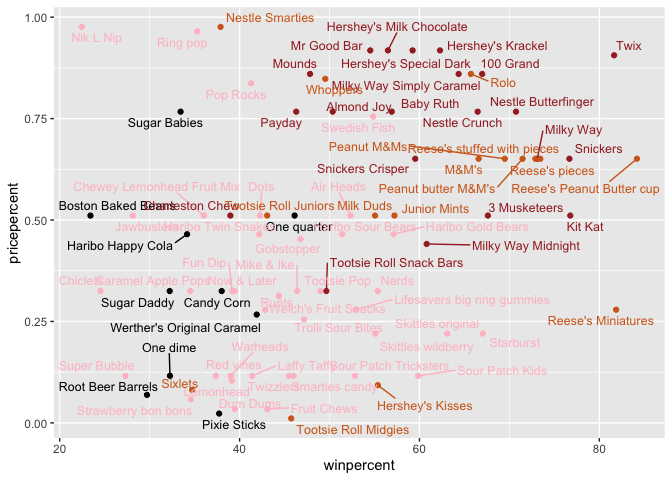
\includegraphics{test_files/figure-latex/unnamed-chunk-57-1.pdf} \#Q19.
Which candy type is the highest ranked in terms of winpercent for the
least money - i.e.~offers the most bang for your buck? Reeses Miniatures

\#Q20. What are the top 5 most expensive candy types in the dataset and
of these which is the least popular? Nik L Nip, Smarties, Ring Pop,
Hersheys Krackel, Hersheys Milk Chocolate. Nik L Nip is the least
popular.

\begin{Shaded}
\begin{Highlighting}[]
\NormalTok{ord }\OtherTok{\textless{}{-}} \FunctionTok{order}\NormalTok{(candy}\SpecialCharTok{$}\NormalTok{pricepercent, }\AttributeTok{decreasing =} \ConstantTok{TRUE}\NormalTok{)}
\FunctionTok{head}\NormalTok{( candy[ord,}\FunctionTok{c}\NormalTok{(}\DecValTok{11}\NormalTok{,}\DecValTok{12}\NormalTok{)], }\AttributeTok{n=}\DecValTok{5}\NormalTok{ )}
\end{Highlighting}
\end{Shaded}

\begin{verbatim}
##                          pricepercent winpercent
## Nik L Nip                       0.976   22.44534
## Nestle Smarties                 0.976   37.88719
## Ring pop                        0.965   35.29076
## Hershey's Krackel               0.918   62.28448
## Hershey's Milk Chocolate        0.918   56.49050
\end{verbatim}

\begin{Shaded}
\begin{Highlighting}[]
\CommentTok{\#install.packages("corrplot")}
\CommentTok{\#library(corrplot)}
\end{Highlighting}
\end{Shaded}

\begin{Shaded}
\begin{Highlighting}[]
\CommentTok{\#cij \textless{}{-} cor(candy)}
\CommentTok{\#corrplot(cij)}
\end{Highlighting}
\end{Shaded}

\#Q22. Examining this plot what two variables are anti-correlated
(i.e.~have minus values)? Chocolate and fruity

\#Q23. Similarly, what two variables are most positively correlated?
Chocolate and winpercent

Section 6

\begin{Shaded}
\begin{Highlighting}[]
\CommentTok{\#pca\textless{}{-}prcomp(candy, scale=TRUE )}
\CommentTok{\#summary(pca)}
\end{Highlighting}
\end{Shaded}

\begin{Shaded}
\begin{Highlighting}[]
\CommentTok{\#plot(pca$x[,1:2])}
\end{Highlighting}
\end{Shaded}

\begin{Shaded}
\begin{Highlighting}[]
\CommentTok{\#plot(pca$x[,1:2], col=my\_cols, pch=16)}
\end{Highlighting}
\end{Shaded}

\begin{Shaded}
\begin{Highlighting}[]
\CommentTok{\# Make a new data{-}frame with our PCA results and candy data}
\CommentTok{\#my\_data \textless{}{-} cbind(candy, pca$x[,1:3])}
\end{Highlighting}
\end{Shaded}

\begin{Shaded}
\begin{Highlighting}[]
\CommentTok{\#p \textless{}{-} ggplot(my\_data) + }
        \FunctionTok{aes}\NormalTok{(}\AttributeTok{x=}\NormalTok{PC1, }\AttributeTok{y=}\NormalTok{PC2, }
            \AttributeTok{size=}\NormalTok{winpercent}\SpecialCharTok{/}\DecValTok{100}\NormalTok{,  }
            \AttributeTok{text=}\FunctionTok{rownames}\NormalTok{(my\_data),}
            \AttributeTok{label=}\FunctionTok{rownames}\NormalTok{(my\_data)) }\SpecialCharTok{+}
        \FunctionTok{geom\_point}\NormalTok{(}\AttributeTok{col=}\NormalTok{my\_cols)}
\end{Highlighting}
\end{Shaded}

\begin{verbatim}
## NULL
\end{verbatim}

\begin{Shaded}
\begin{Highlighting}[]
\CommentTok{\#p}
\end{Highlighting}
\end{Shaded}

\begin{Shaded}
\begin{Highlighting}[]
\CommentTok{\#library(ggrepel)}

\CommentTok{\#p + geom\_text\_repel(size=3.3, col=my\_cols, max.overlaps = 7)  + }
 \CommentTok{\# theme(legend.position = "none") +}
  \CommentTok{\#labs(title="Halloween Candy PCA Space",}
       \CommentTok{\#subtitle="Colored by type: chocolate bar (dark brown), chocolate other (light  brown), fruity (red), other (black)",}
       \CommentTok{\#caption="Data from 538")}
\end{Highlighting}
\end{Shaded}

\begin{Shaded}
\begin{Highlighting}[]
\CommentTok{\#library(plotly)}
\CommentTok{\#ggplotly(p)}
\end{Highlighting}
\end{Shaded}

\begin{Shaded}
\begin{Highlighting}[]
\CommentTok{\#par(mar=c(8,4,2,2))}
\CommentTok{\#barplot(pca$rotation[,1], las=2, ylab="PC1 Contribution")}
\end{Highlighting}
\end{Shaded}

Q24. What original variables are picked up strongly by PC1 in the
positive direction? Do these make sense to you?

Fruity, hard, pluribus. Most fruity candies are hard and pluribus so it
makes sense that those would be clustered similarly.

\begin{Shaded}
\begin{Highlighting}[]
\FunctionTok{rownames}\NormalTok{(candy)}
\end{Highlighting}
\end{Shaded}

\begin{verbatim}
##  [1] "100 Grand"                   "3 Musketeers"               
##  [3] "One dime"                    "One quarter"                
##  [5] "Air Heads"                   "Almond Joy"                 
##  [7] "Baby Ruth"                   "Boston Baked Beans"         
##  [9] "Candy Corn"                  "Caramel Apple Pops"         
## [11] "Charleston Chew"             "Chewey Lemonhead Fruit Mix" 
## [13] "Chiclets"                    "Dots"                       
## [15] "Dum Dums"                    "Fruit Chews"                
## [17] "Fun Dip"                     "Gobstopper"                 
## [19] "Haribo Gold Bears"           "Haribo Happy Cola"          
## [21] "Haribo Sour Bears"           "Haribo Twin Snakes"         
## [23] "Hershey's Kisses"            "Hershey's Krackel"          
## [25] "Hershey's Milk Chocolate"    "Hershey's Special Dark"     
## [27] "Jawbusters"                  "Junior Mints"               
## [29] "Kit Kat"                     "Laffy Taffy"                
## [31] "Lemonhead"                   "Lifesavers big ring gummies"
## [33] "Peanut butter M&M's"         "M&M's"                      
## [35] "Mike & Ike"                  "Milk Duds"                  
## [37] "Milky Way"                   "Milky Way Midnight"         
## [39] "Milky Way Simply Caramel"    "Mounds"                     
## [41] "Mr Good Bar"                 "Nerds"                      
## [43] "Nestle Butterfinger"         "Nestle Crunch"              
## [45] "Nik L Nip"                   "Now & Later"                
## [47] "Payday"                      "Peanut M&Ms"                
## [49] "Pixie Sticks"                "Pop Rocks"                  
## [51] "Red vines"                   "Reese's Miniatures"         
## [53] "Reese's Peanut Butter cup"   "Reese's pieces"             
## [55] "Reese's stuffed with pieces" "Ring pop"                   
## [57] "Rolo"                        "Root Beer Barrels"          
## [59] "Runts"                       "Sixlets"                    
## [61] "Skittles original"           "Skittles wildberry"         
## [63] "Nestle Smarties"             "Smarties candy"             
## [65] "Snickers"                    "Snickers Crisper"           
## [67] "Sour Patch Kids"             "Sour Patch Tricksters"      
## [69] "Starburst"                   "Strawberry bon bons"        
## [71] "Sugar Babies"                "Sugar Daddy"                
## [73] "Super Bubble"                "Swedish Fish"               
## [75] "Tootsie Pop"                 "Tootsie Roll Juniors"       
## [77] "Tootsie Roll Midgies"        "Tootsie Roll Snack Bars"    
## [79] "Trolli Sour Bites"           "Twix"                       
## [81] "Twizzlers"                   "Warheads"                   
## [83] "Welch's Fruit Snacks"        "Werther's Original Caramel" 
## [85] "Whoppers"
\end{verbatim}

\begin{Shaded}
\begin{Highlighting}[]
\FunctionTok{rownames}\NormalTok{(candy)}\OtherTok{\textless{}{-}}\FunctionTok{gsub}\NormalTok{(}\StringTok{"Õ"}\NormalTok{,}\StringTok{"\textquotesingle{}"}\NormalTok{, }\FunctionTok{rownames}\NormalTok{(candy))}
\end{Highlighting}
\end{Shaded}


\end{document}
